\label{corpus}
\minitoc
\section{Description du corpus Charcot}
Le fonds patrimonial de Jean-Martin Charcot est conservé à la Bibliothèque de Neurosciences Jean-Martin Charcot par la BSU.
%\footnote{\url{https://www.sorbonne-universite.fr/bu/decouvrir-nos-bibliotheques/la-bibliotheque-charcot}.}
 Ce fonds regroupe des ouvrages suivants : 
\begin{itemize}
\item fonds historique Charcot (bibliothèque personnelle de Charcot) : ouvrages, périodiques, collection de thèses et de tirés à part, manuscrits, observations, collection neurologique couvrant la seconde partie du XIX\ieme{} siècle, fonds bibliophilique ancien ;
\item collections de la bibliothèque des Internes de la Salpêtrière : ouvrages, périodiques, thèses en neurologie et psychiatrie pour la période 1800-1950 ;
\item donations en ouvrages du docteur Achille Souques.
\end{itemize}
\medskip
Dans un souci de préservation d'ouvrages originaux et de valorisation de collections ayant un caractère iconographique notable, une partie de ce fonds a été numérisée. Ces archives numérisées sont disponibles sur le portail numérique
SorbonNum\footnote{anc. Jubilothèque, \url{https://patrimoine.sorbonne-universite.fr/collection/Fonds-Charcot}}, porte d'entrée unique vers les collections scientifiques patrimoniales et numériques de Sorbonne Université, ainsi que sur Gallica, bibliothèque numérique de la Bibliothèque nationale de France (\textsc{BnF})\footnote{\url{https://gallica.bnf.fr/services/engine/search/sru?operation=searchRetrieve&version=1.2&query=\%28gallica\%20all\%20\%22Charcot\%2C\%20Jean-Martin\%22\%29&lang=fr&suggest=0}.}.

Le fonds numérisé a été décrit et divisé par la BSU en quatre grandes typologies de documents :
\begin{enumerate}
\item \underline{Fonds iconographique}
\begin{itemize}
\item \textbf{Album des internes} : Album des promotions annuelles d'internes, photographiées et classées par établissements de l'Assistance Publique, entre 1860 et 1963 ;
\item \textbf{Photographies sur les aliénés de Bicêtre par Désiré Magloire Bourneville} : deux albums présentant les photographies des \og{}petits enfants anormaux\fg{} hospitalisés à Bicêtre dans le service du docteur Bourneville, collaborateur de Charcot.
\end{itemize}
\item \underline{Leçons et manuscrits des leçons de Charcot}
\begin{itemize}
\item \textbf{Manuscrits des leçons et observations de Charcot (1825-1893)} : leçons orales de Charcot, rédigées intégralement de sa main et annotées ;
\item \textbf{Leçons de Charcot} : numérisation des volumes de l'\textit{\OE{}uvre Complète} de Charcot consacrés au système nerveux et à l'enseignement clinique, comme par exemple les célèbres leçons du Mardi, sur l'hystérie notamment.
\end{itemize}
\item \underline{Périodiques}
\begin{itemize}
\item \textbf{\textit{Les Recherches cliniques et thérapeutiques sur l'épilepsie, l'hystérie et l'idiotie (1872 -1903)}} de Bourneville. Y est retracée toute l'activité du Service des Enfants Idiots, à la Salpêtrière puis à Bicêtre, par le biais des compte-rendu illustrés de photographies et rédigés par Bourneville ;
\item \textbf{\textit{Revue de l'Hypnotisme (1887-1910)}} : périodique consacré à l'hypnotisme que Charcot a réhabilité, publiant les principaux articles théoriques sur cette discipline ;
\item \textbf{\textit{Journal du magnétisme (1845-1861)}} : la collection reflète les recherches sur le magnétisme, renouvelées au milieu du XIX\ieme{} siècle ; 
\item \textbf{\textit{Revue photographique des hôpitaux de Paris (1869-1872)}}. Première revue exposant les applications de la photographie à la médecine, notamment la médecine hospitalière, à travers les études menées à l'Hôpital Saint Louis, et à la Salpêtrière ;
\item \textbf{\textit{Iconographie Photographique de la Salpêtrière (1875-1879)}}. La collection présente les observations de patientes examinées à la Salpêtrière, accompagnées de photographies d'Albert Londe, présentant les divers stades de la crise d'hystérie ;
\item \textbf{\textit{Nouvelle Iconographie de la Salpêtrière (1888-1918)}}. La revue est fondée sous la direction de Charcot par Paul Richer, Gilles de la Tourette et Albert Londe, directeur du service photographique. Elle réunit la collection de clichés constituée à la Salpêtrière a pour but la représentation objective des pathologies observées. Elle prend la relève de l'\textit{Iconographie Photographique de la Salpêtrière}. Les articles sont illustrés de photographies, de dessins et de lithographies ;
\item \textbf{\textit{Archives de neurologie (1880-1907)}}. Sous-titrée \og{}Revue trimestrielle des maladies nerveuses et mentales\fg{}, les Archives de neurologie sont publiées sous la direction de Charcot par Bourneville. La revue édite, groupe, catégorise et compare la masse des travaux de pathologie nerveuse. Les \textit{Archives de neurologie} sont devenues bisannuelles en 1881.
\end{itemize}
\item \underline{Ouvrages de la bibliothèque de Charcot}
\begin{itemize}
\item \textbf{Collection d'atlas d'anatomie et de pathologie du système nerveux}, publiés durant le XIX\ieme{} siècle. L'iconographie de ces ouvrages est remarquable, à commencer par l'\textit{Atlas de Vicq d'Azyr}, médecin du roi Louis XVI ;
\item \textbf{Traités}. Cette collection regroupe à la fois des traités sélectionnés dans la bibliothèque de Charcot (comme l'\textit{Opera omnia}$\dots$ de Thomas Willis, 1682, comportant des gravures), des atlas et des textes significatifs des successeurs de Charcot, issus de la bibliothèque des Internes de la Salpêtrière (par exemple l'\textit{Anatomie des centres nerveux} des Déjerine).
\end{itemize}
\end{enumerate}



\section{Constitution du corpus Charcot}
Le corpus de travail est constitué de 201 documents OCRisés, sans post-correction, gracieusement fournis au format \textsc{XML} par la \textsc{BSU}\footnote{À cette occasion, je remercie chaleureusement M\textsuperscript{me} Adeline Batailler, chargée de la valorisation et de l'évaluation des collections du département des Collections de la \textsc{BSU}, pour ses conseils précieux concernant le fonds Charcot.}. Originalement, ces fichiers contenaient seulement les balises \texttt{<doc>} (document comme objet), \texttt{<id\_doc>} (identifiant du document) et \texttt{<pages>} (pages du document). C'est pourquoi nous avons restructuré les textes au format \textsc{XML-TEI}, à l'aide de l’outil dédié intégré à \textsc{Pandore}\footnote{\url{https://obtic-gpu1.mesu.sorbonne-universite.fr:8550/conversion_xml}}, une boîte à outils développée par l'équipe ObTIC et hébergée par Sorbonne Université. L'encodage du corpus selon le format \textsc{XML-TEI} a été effectué en s'appuyant sur le modèle illustré dans le code \ref{lst:model_obvie}, ce qui a rendu possible l'indexation et la publication du corpus Charcot en ligne \textit{via} le logiciel \textsc{OBVIE}\footnote{\url{https://obtic.huma-num.fr/obvie/charcot/?view=corpus}} \citep{alrahabi2022obvie}. En plus de la plateforme \textsc{OBVIE}, le corpus est librement disponible et interrogeable sur la plateforme \textsc{TextPair}\footnote{\url{https://anomander.uchicago.edu/}} (voir la partie \ref{sect:obvie_textpair}).
\begin{listing}[h]
	\caption{Modèle du document \textsc{XML-TEI} requis pour sa publication sur la plateforme \textsc{OBVIE}.}
	\label{lst:model_obvie}
\begin{minted}[%
	bgcolor=codebg,
	linenos,
	breaklines,
	fontsize=\small,
	tabsize=2,
	obeytabs,
	xleftmargin=1em
	]{xml}
<?xml version="1.0" encoding="UTF-8"?>
<?xml-stylesheet type="text/xsl" href="../../Teinte/tei2html.xsl"?>
<TEI xmlns="http://www.tei-c.org/ns/1.0">
  <teiHeader>
    <fileDesc>
      <titleStmt>
        <title>mon titre</title>
        <author>mon auteur</author>
      </titleStmt>
    </fileDesc>
    <profileDesc>
      <creation>
        <date when="1890"></date>
      </creation>
    </profileDesc>
  </teiHeader>
  <text>
    <body>
      <div>
        <p>
          <s>Une phrase.</s>
          <s>Une autre phrase.</s>
        </p>
      </div>
    </body>
  </text>
</TEI>
\end{minted}
\end{listing}


%Afin de mesurer l'impact de Charcot sur son entourage et d'analyser la circulation de concepts véhiculés dans le corpus, 

Afin de mieux distinguer les auteurs des ouvrages composant notre corpus, nous avons séparé les textes rédigés par Charcot de ceux écrits par ses co-auteurs (p. ex. Bourneville) ou ses élèves (comme Gilles de la Tourette). Nous avons obtenu respectivement 68 (corpus \og{}Charcot\fg{}) et 133 (corpus \og{}Autres\fg{}) documents, comme présenté dans le tableau \ref{tab:corpus}.


% Please add the following required packages to your document preamble:
% \usepackage{booktabs}
\begin{table}[h]
	\small
	\centering
	\resizebox{\textwidth}{!}{  
		\begin{tabular}{@{}crrrrrrr@{}}
			\toprule
			\textbf{Corpus}  & \multicolumn{1}{c}{\textbf{Ouvrages}} & \multicolumn{1}{c}{\textbf{Tokens}} & \multicolumn{1}{c}{\textbf{\%}} & 
			\multicolumn{1}{c}{\textbf{Types}} &
			\multicolumn{1}{c}{\textbf{Lemmes}} & \multicolumn{1}{c}{\textbf{Diversité (\%)}} & \multicolumn{1}{c}{\textbf{Mémoire (en Mo)}}\\ \midrule
			Charcot & 68                            & 15 025 612 & 38,27 & 1 147 371 & 809 611 & 7,64  & 130,9      \\ \midrule
			Autres  & 133                           & 24 232 207 & 61,73  & 1 773 538 & 1 218 074 & 7,32 & 179,6   \\ \midrule
			\textbf{Total}  & \textbf{201}                           & \textbf{39 257 819} & 100 & 2 920 909 & 2 027 685 & 14,96 & 310,5   \\ \bottomrule
		\end{tabular}
	}
	\caption{Description de notre corpus d'étude.}
	\label{tab:corpus}
\end{table}

Il convient néanmoins de préciser que le corpus Charcot inclut les ouvrages auxquels Charcot a contribué en tant que co-auteur, en raison de leur nature collaborative, tandis que le corpus Autres regroupe des ouvrages rédigés sans sa participation. Le sous-corpus consacré aux textes médicaux de Charcot constitue 38,27 \% de l’ensemble du corpus, correspondant à 15 025 612 tokens. En comparaison, le sous-corpus médical regroupant les écrits d'autres scientifiques représente 61,73 \% du corpus total, soit 24 232 207 tokens (le tokeniseur provient du modèle français large \texttt{fr\_core\_news\_lg} de l'outil \texttt{spaCy}\footnote{\url{https://spacy.io/models/fr\#fr_core_news_lg}}). Le corpus est assez volumineux, tant par son nombre de tokens (39 257 819 millions au total) que par l'espace mémoire qu'il occupe (206,3 Mo). La diversité lexicale a été déterminée en calculant le ratio entre les types et les tokens, les types correspondant aux mots distincts. Nous constatons un vocabulaire relativement limité en termes de mesures telle que celle-ci (diversité lexicale de 7,64 \% et de 7,32 \% pour le corpus Charcot et le corpus Autres, respectivement), ce qui suggère une répétition fréquente des termes scientifiques. Cette faible diversité lexicale est effectivement caractéristique des textes scientifiques, où l'utilisation répétée de termes spécifiques est essentielle pour assurer la précision et la clarté.



\begin{figure}[htp]
	\centering
	
	\begin{subfigure}[t]{0.3\textwidth}
		\centering
		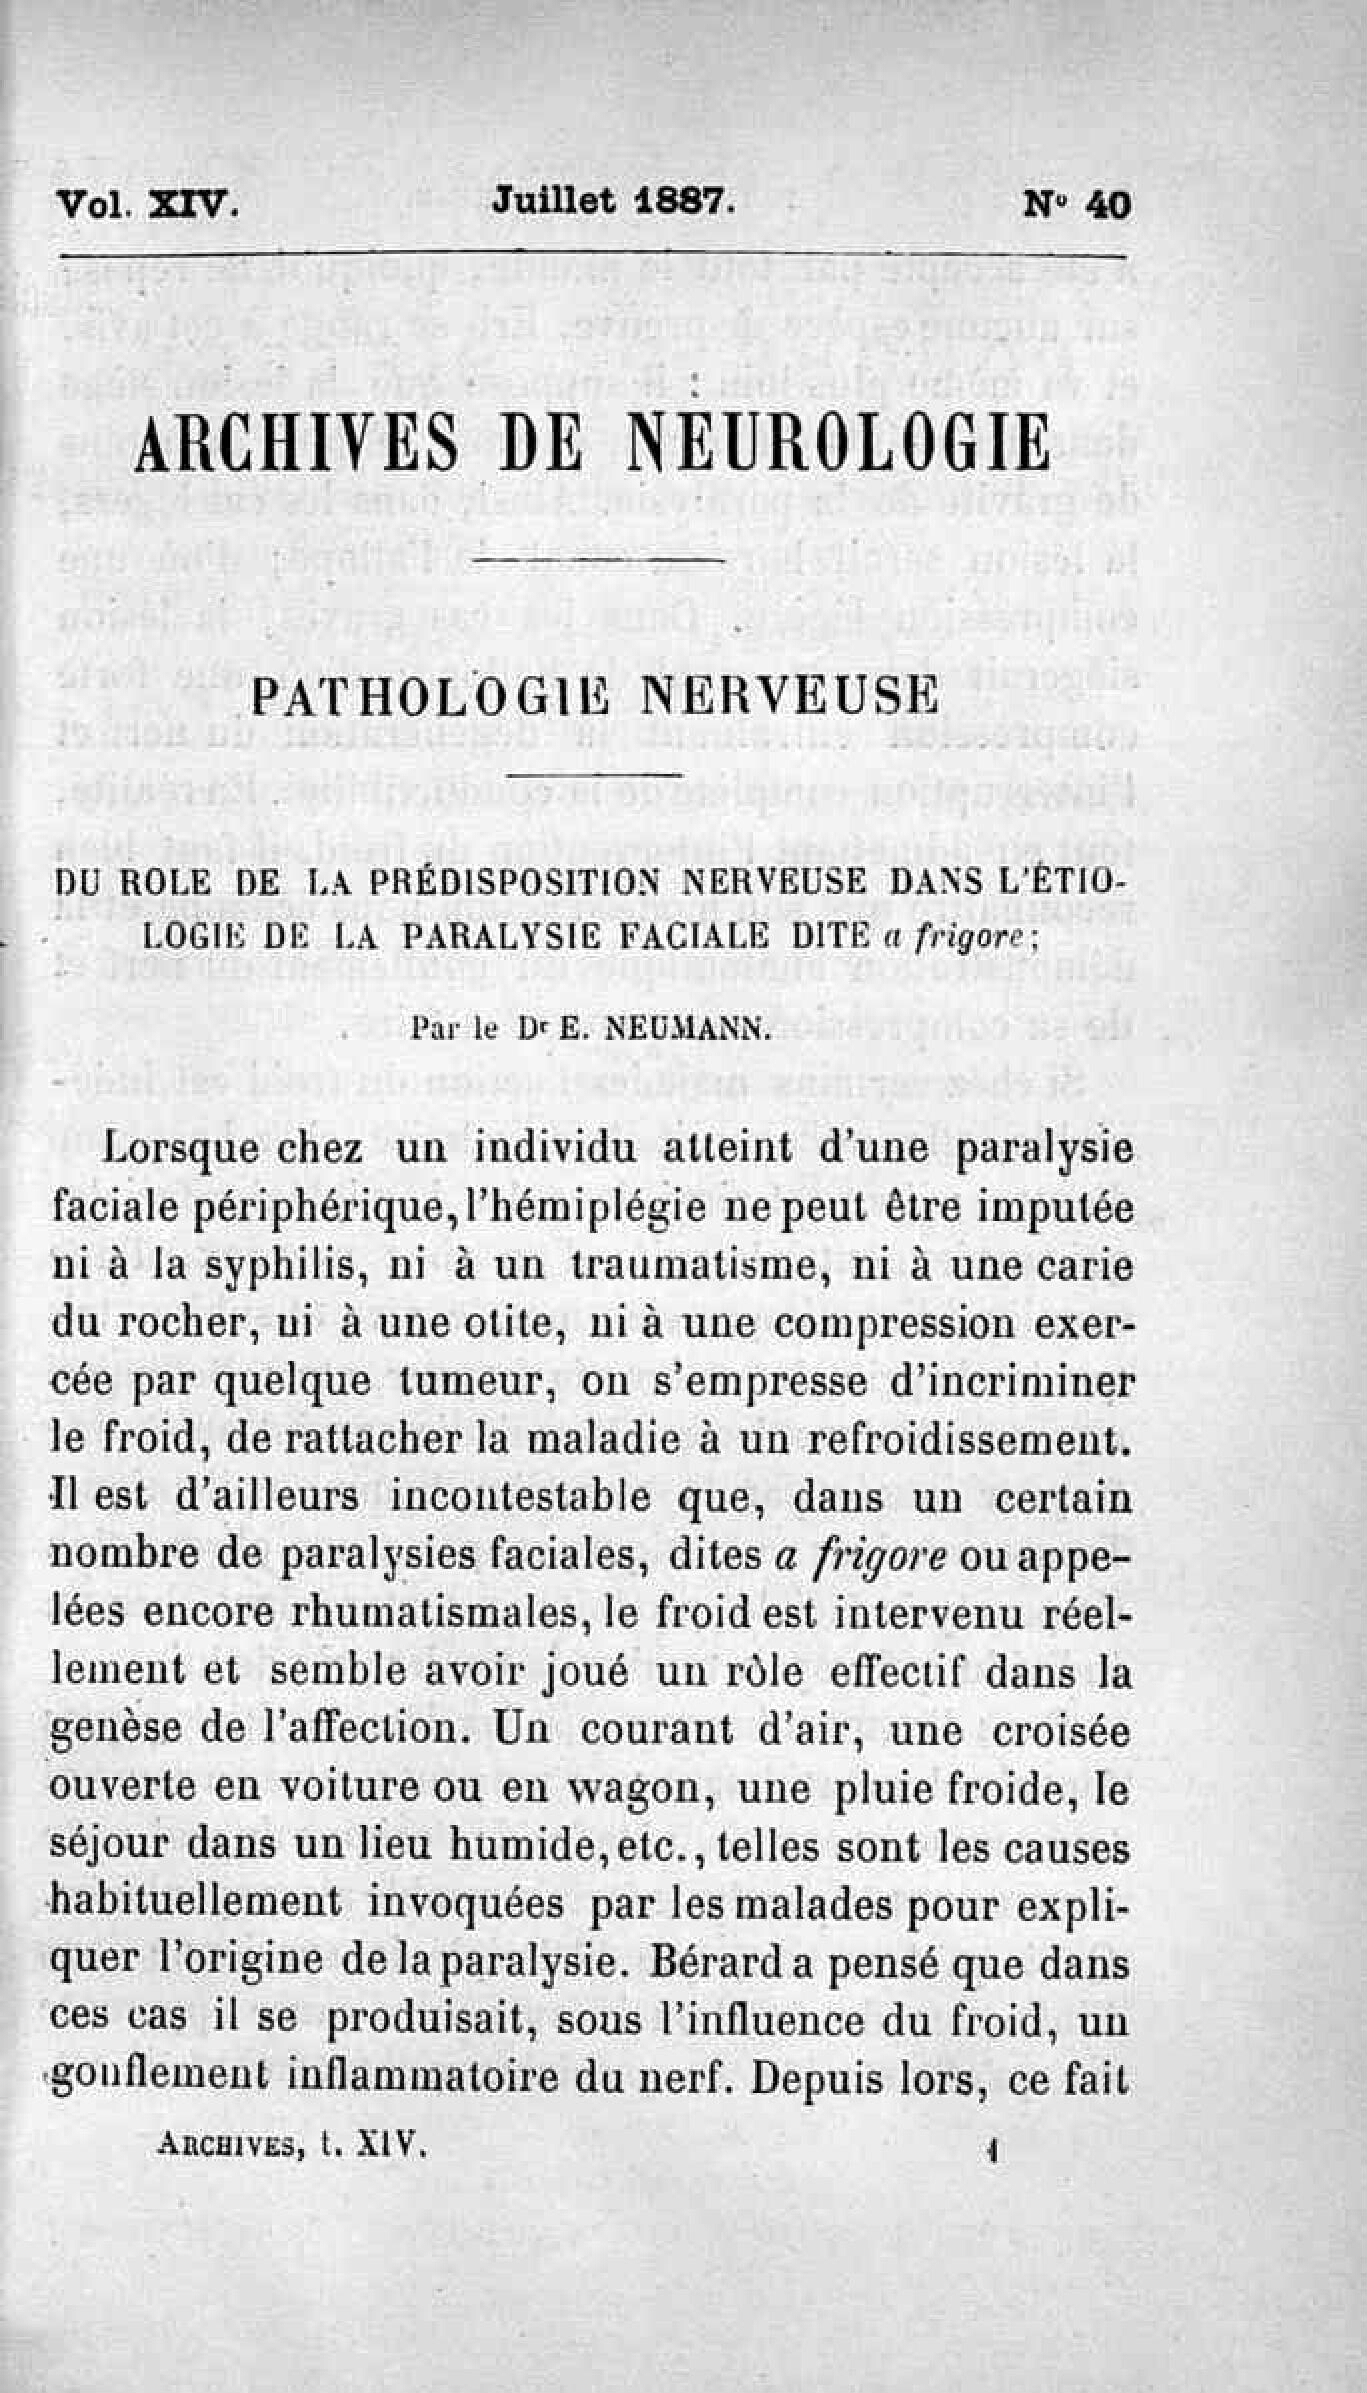
\includegraphics[height=6cm]{img/archives_neurologie.jpg}
		\caption{Charcot, J.-M., \& Bourneville, D. M. (1881). \textit{Archives de neurologie [Tome 01] : revue trimestrielle des maladies nerveuses et mentales}. Bureaux du progrès médical (Paris).}
	\end{subfigure}\hfill
	\begin{subfigure}[t]{0.3\textwidth}
		\centering
		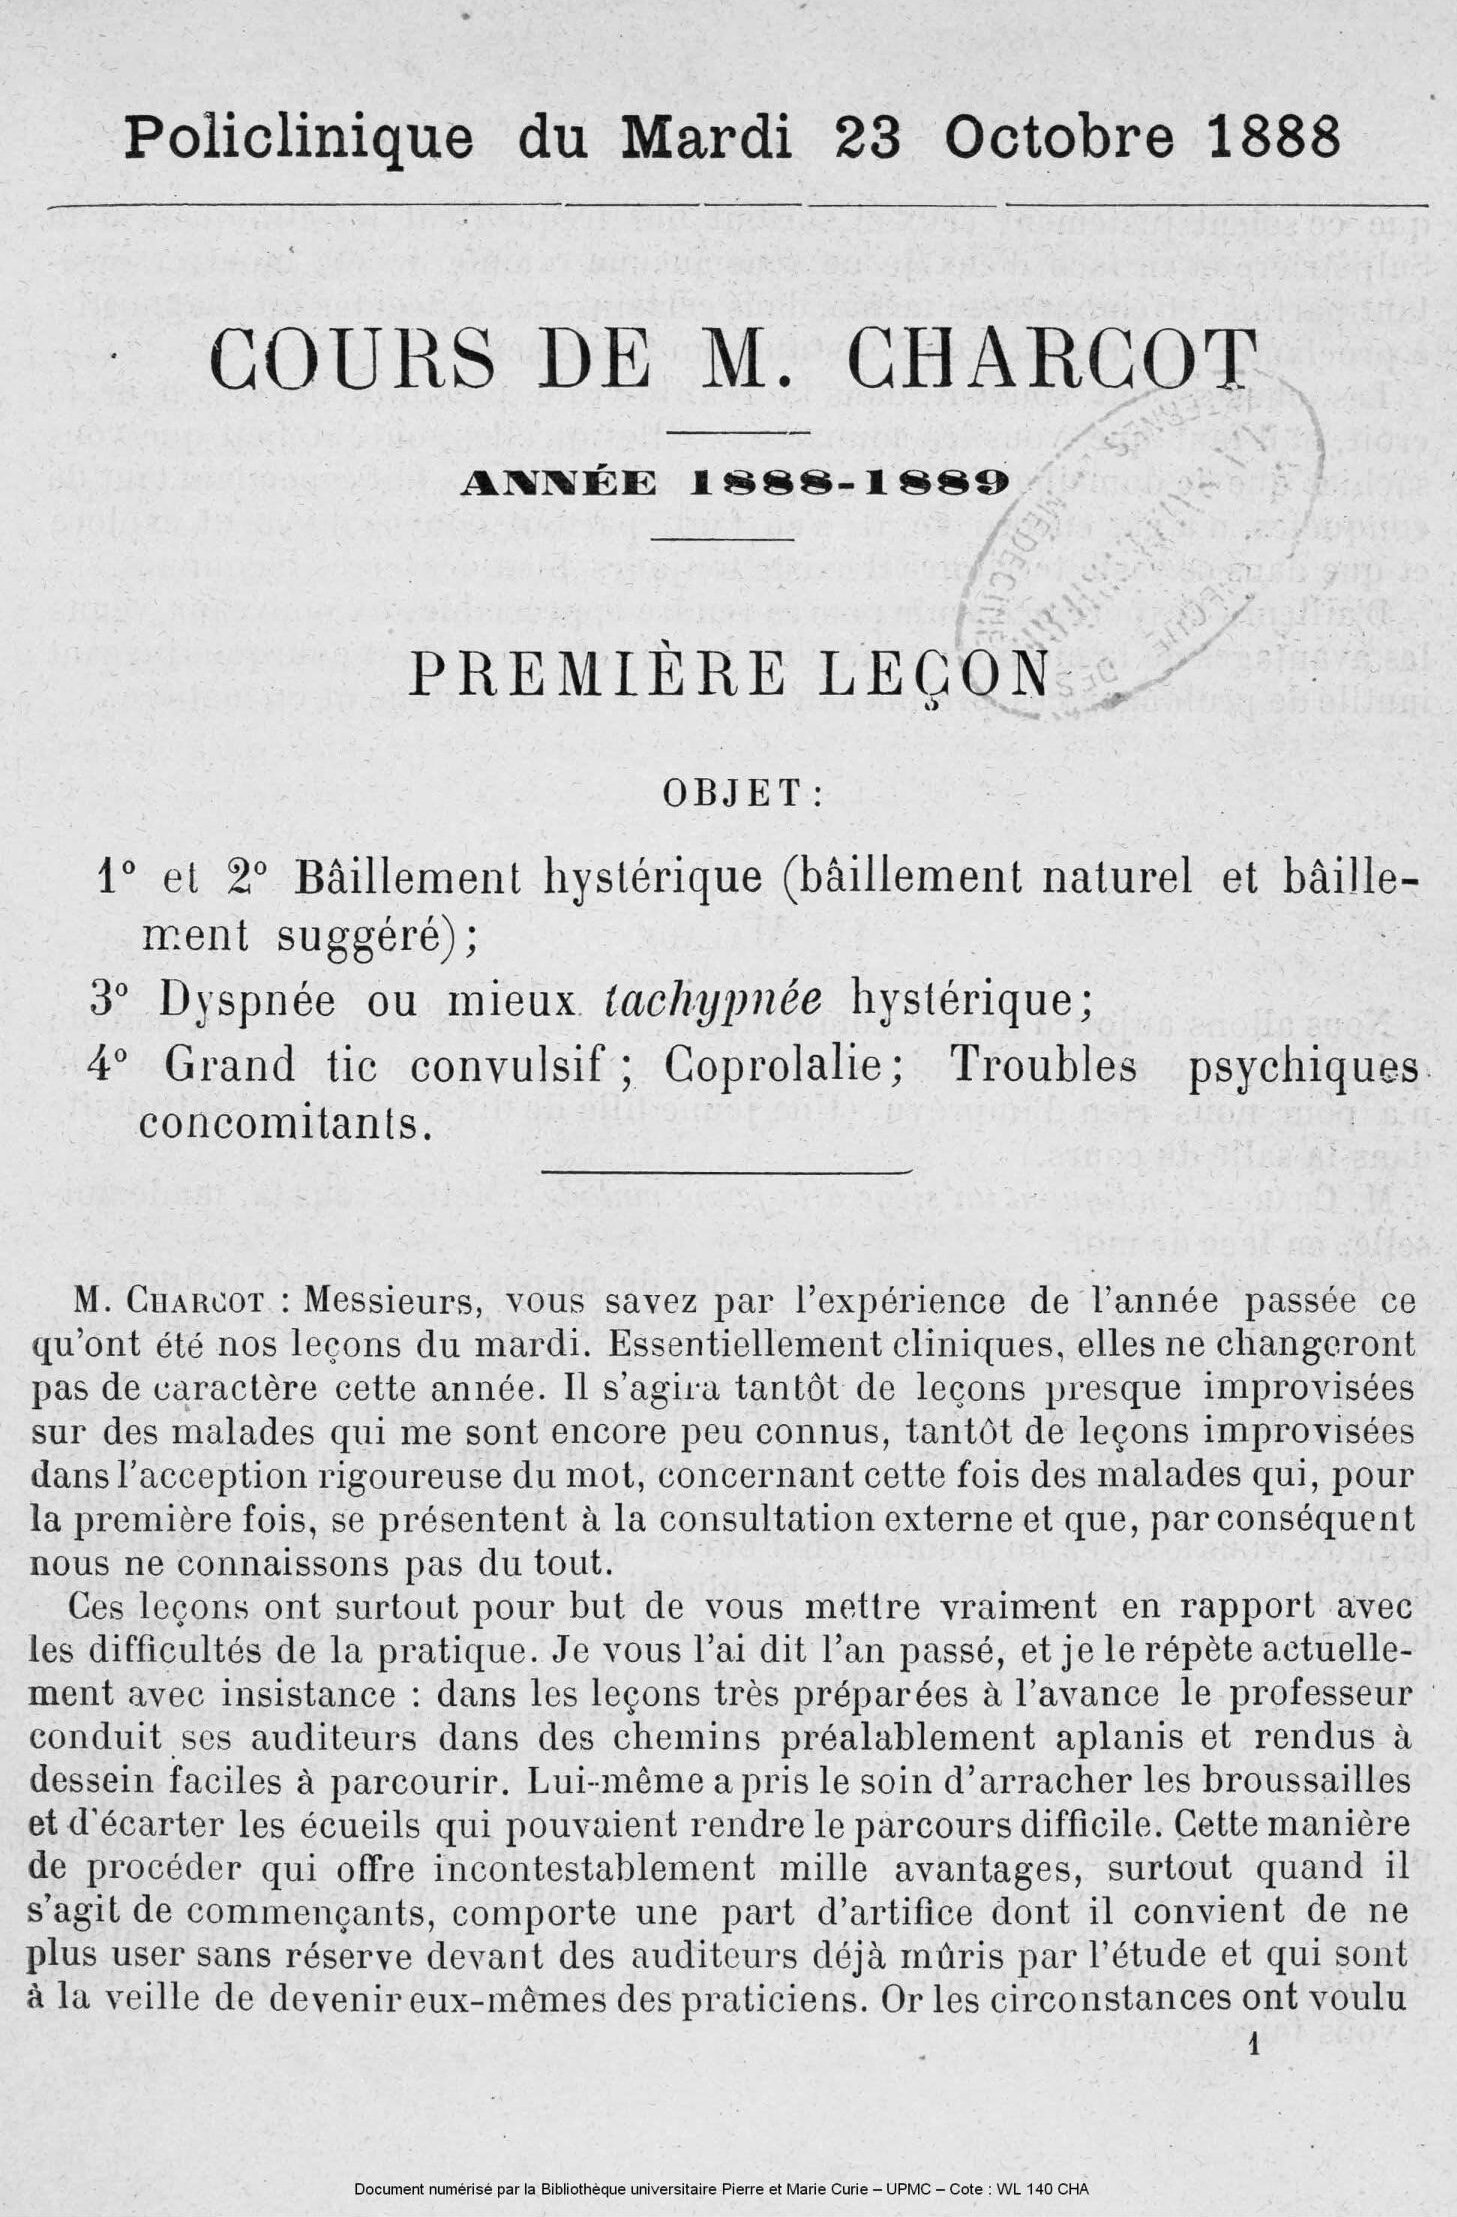
\includegraphics[height=6cm]{img/lecons.jpg}
		\caption{Blin, E., Colin, H., Charcot, J.-M., \& Charcot, J.-B. (1889). \textit{Leçons du Mardi à la Salpêtrière. Policlinique 1888-1889}. A. Delahaye \& E. Lecrosnier (Paris). Bureaux du progrès médical (Paris).}
	\end{subfigure}
	\hfill
		\begin{subfigure}[t]{0.3\textwidth}
		\centering
		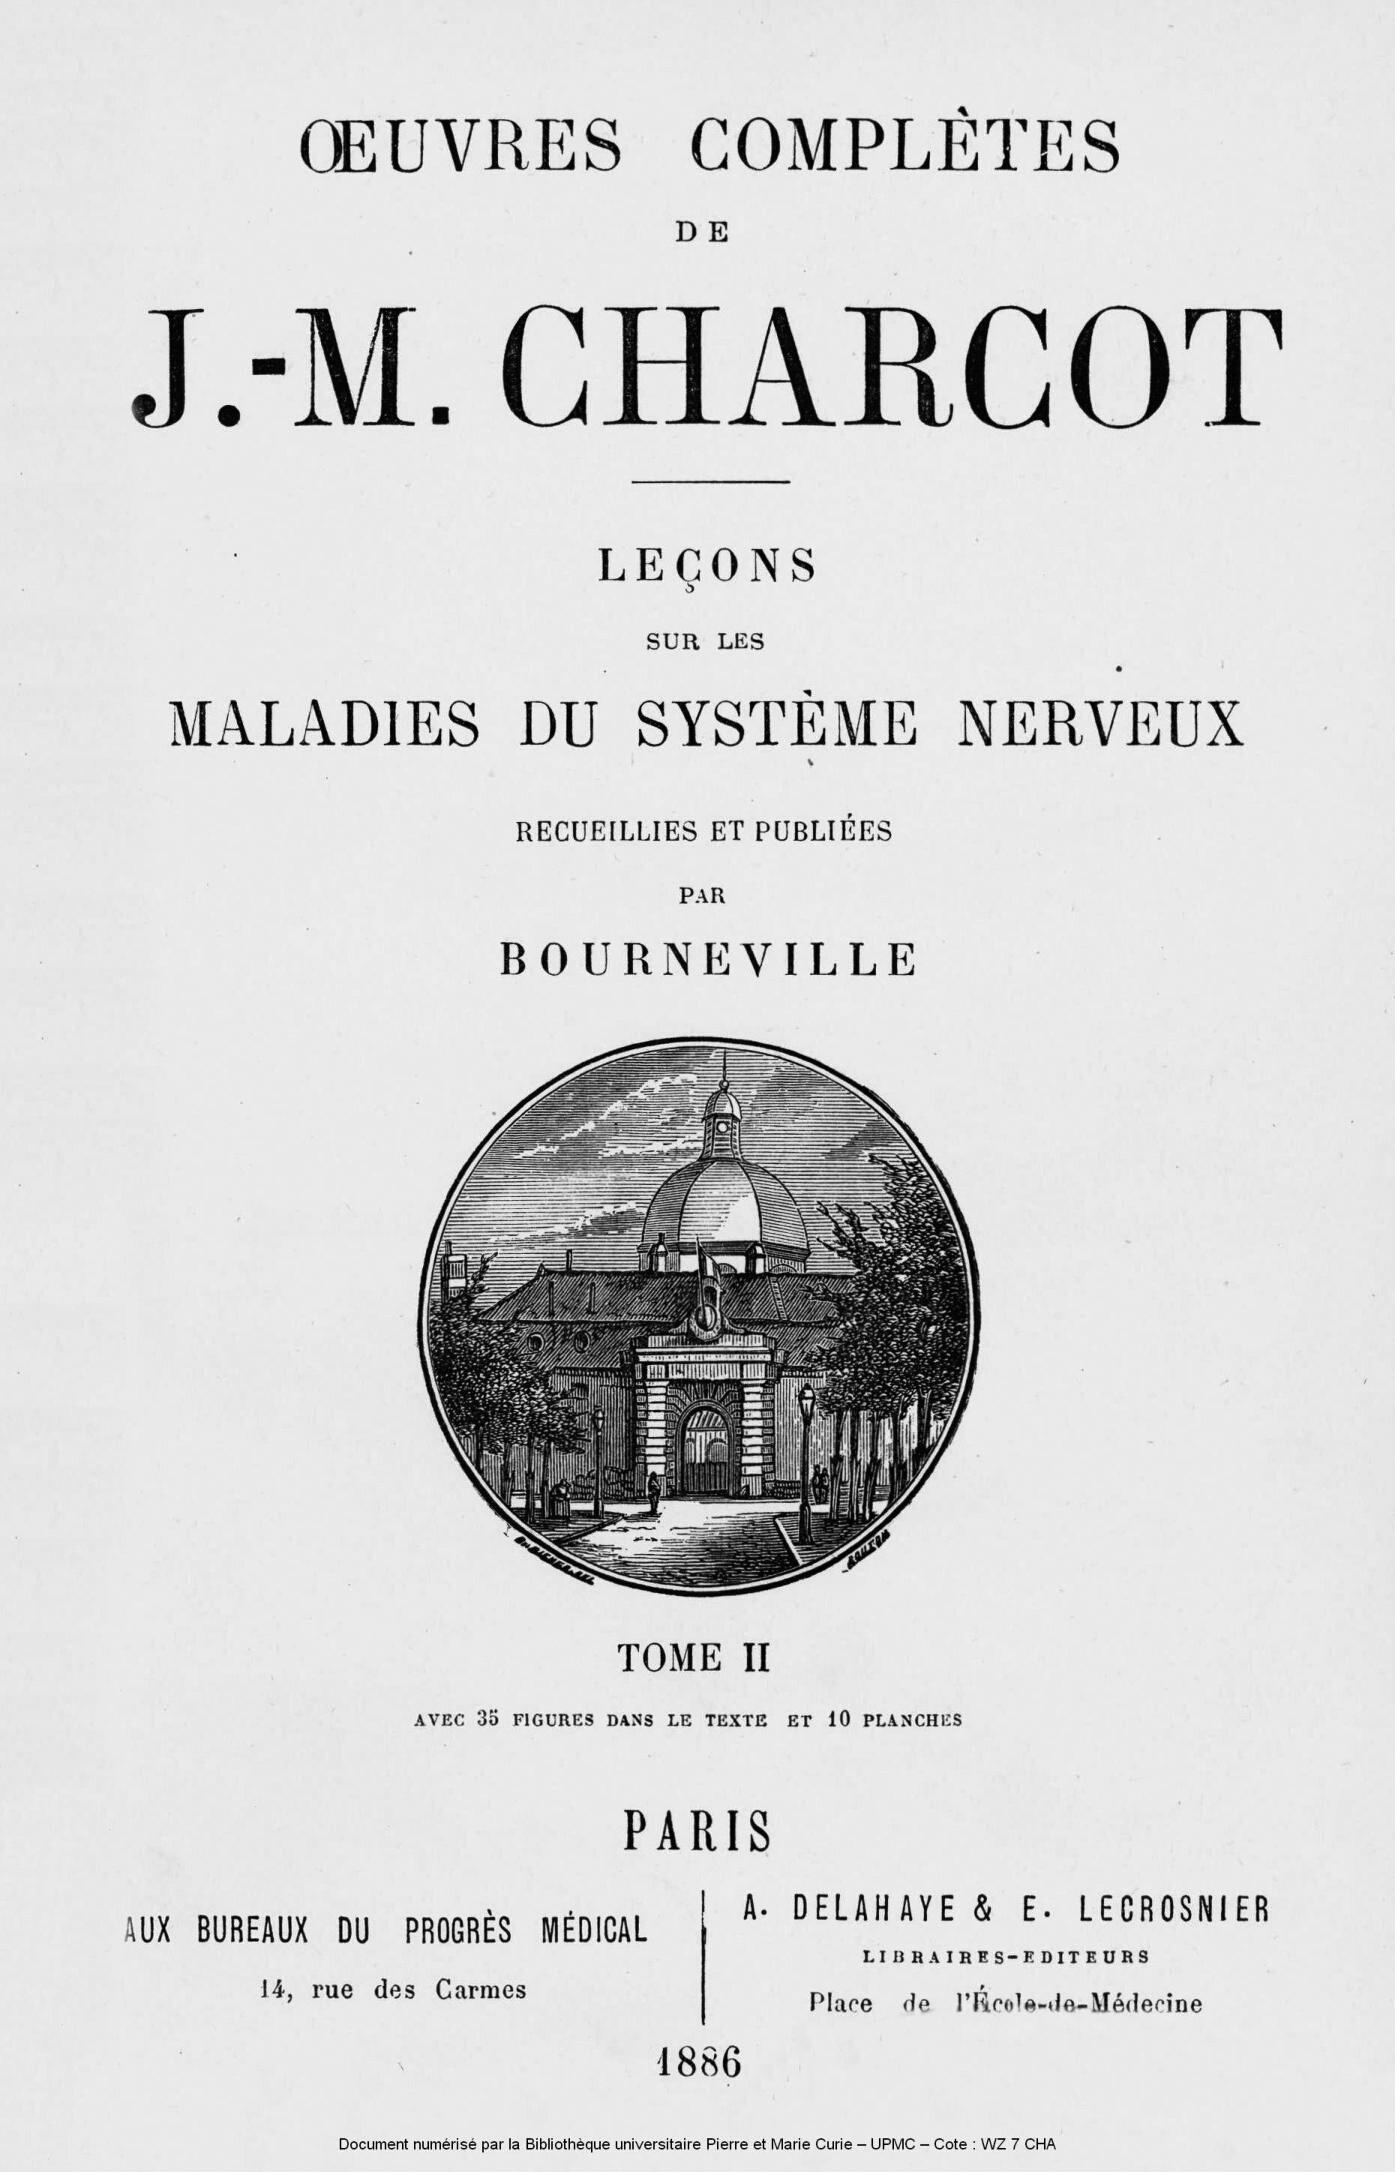
\includegraphics[height=6cm]{img/oeuvres_completes.jpg}
		\caption{Bourneville, D. M., \& Charcot, J.-M. (1892). \textit{\OE{}uvres complètes de J. M. Charcot. Tome 1. Leçons sur les maladies du système nerveux}. Bureaux du progrès médical (Paris).}
	\end{subfigure}
	\caption{Trois exemples de pages issues du corpus Charcot.}
	\label{fig:charcot_pages}
\end{figure}


\begin{figure}[htp]
	\centering
	
	\begin{subfigure}[t]{0.3\textwidth}
		\centering
		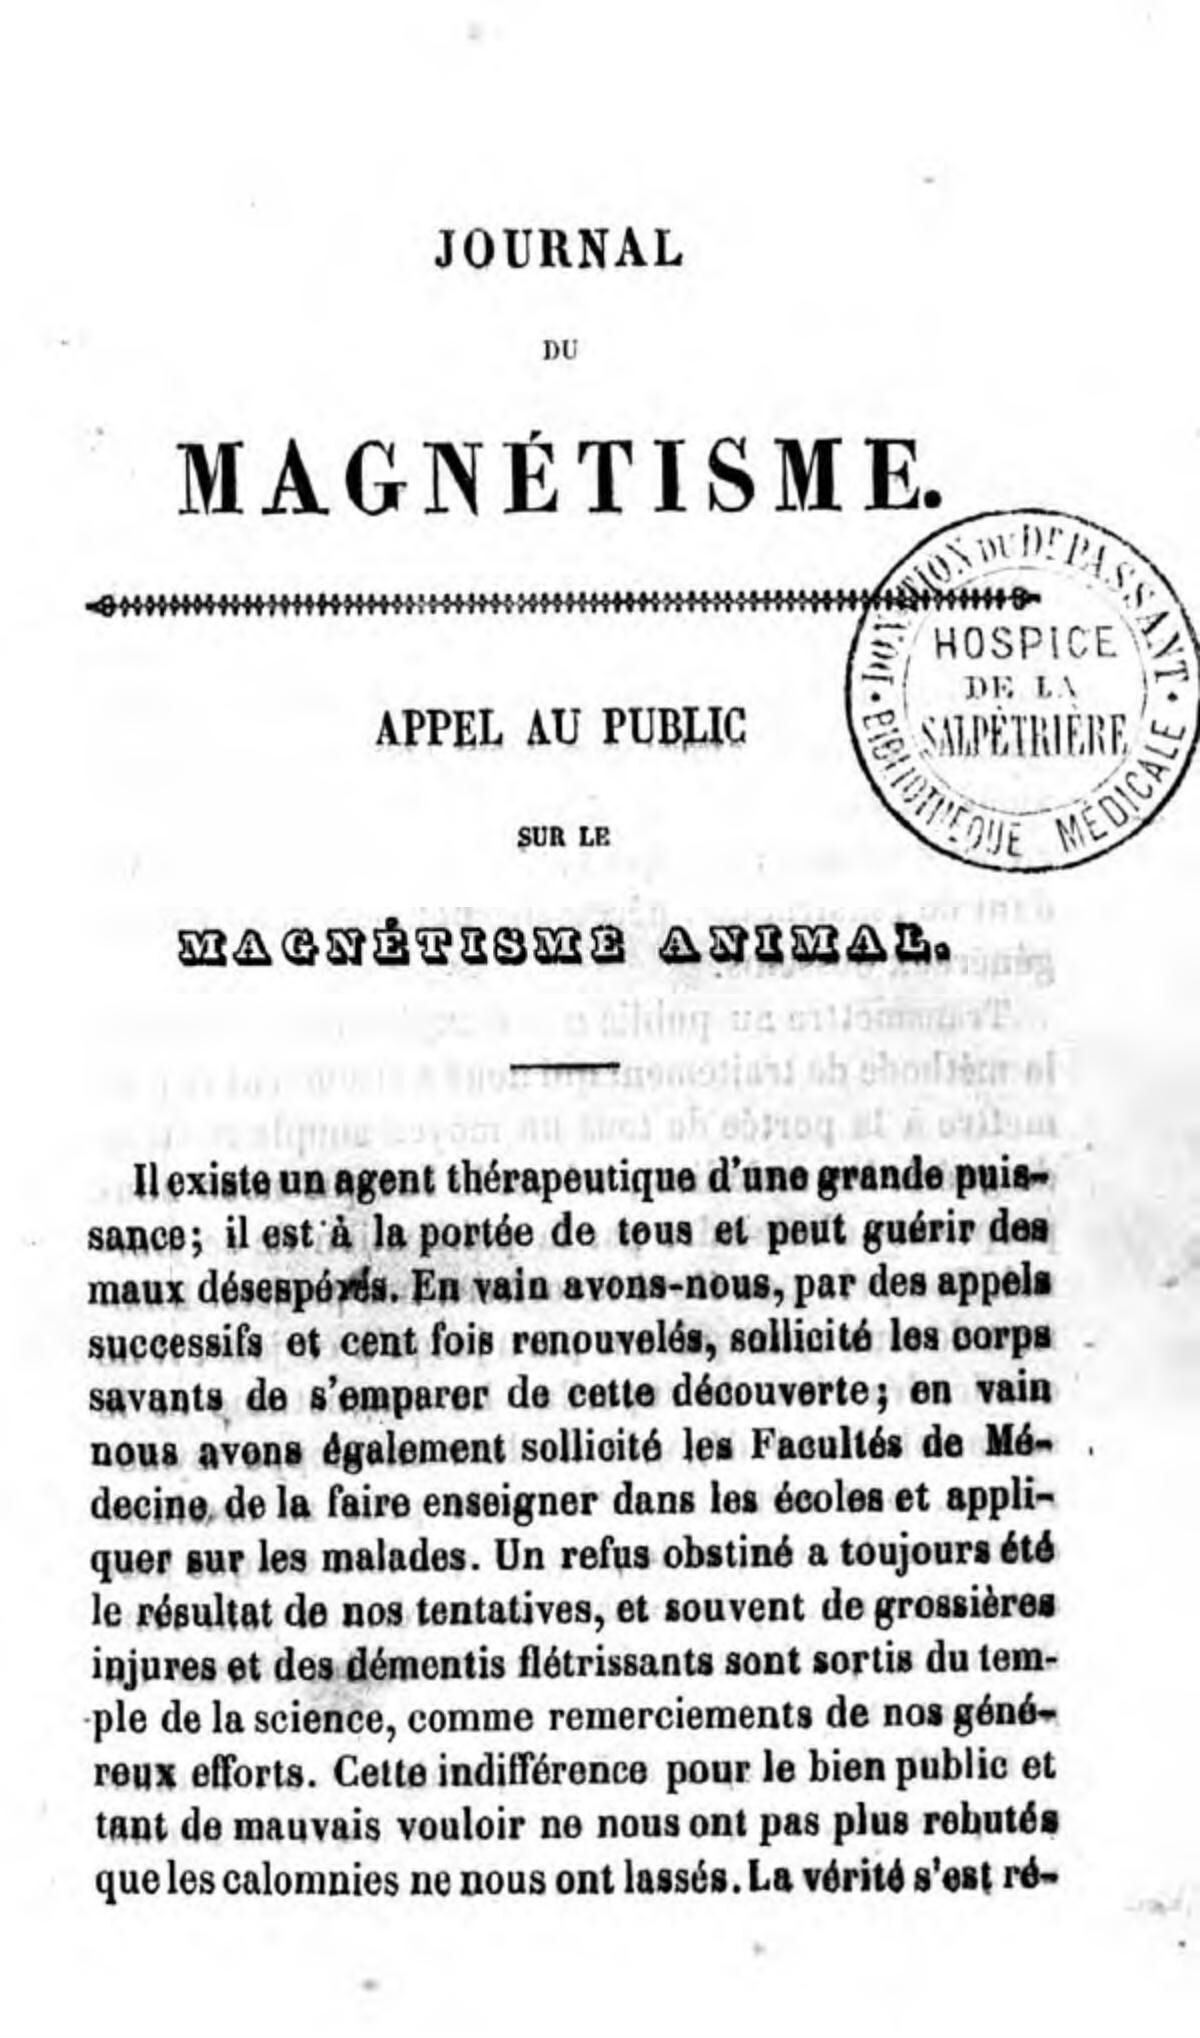
\includegraphics[height=6cm]{img/magnetisme.jpg}
		\caption{Société de magnétiseurs et de médecins. (1845). \textit{Journal du magnétisme [Tome I]}. A. René (Paris).}
	\end{subfigure}\hfill
	\begin{subfigure}[t]{0.3\textwidth}
		\centering
		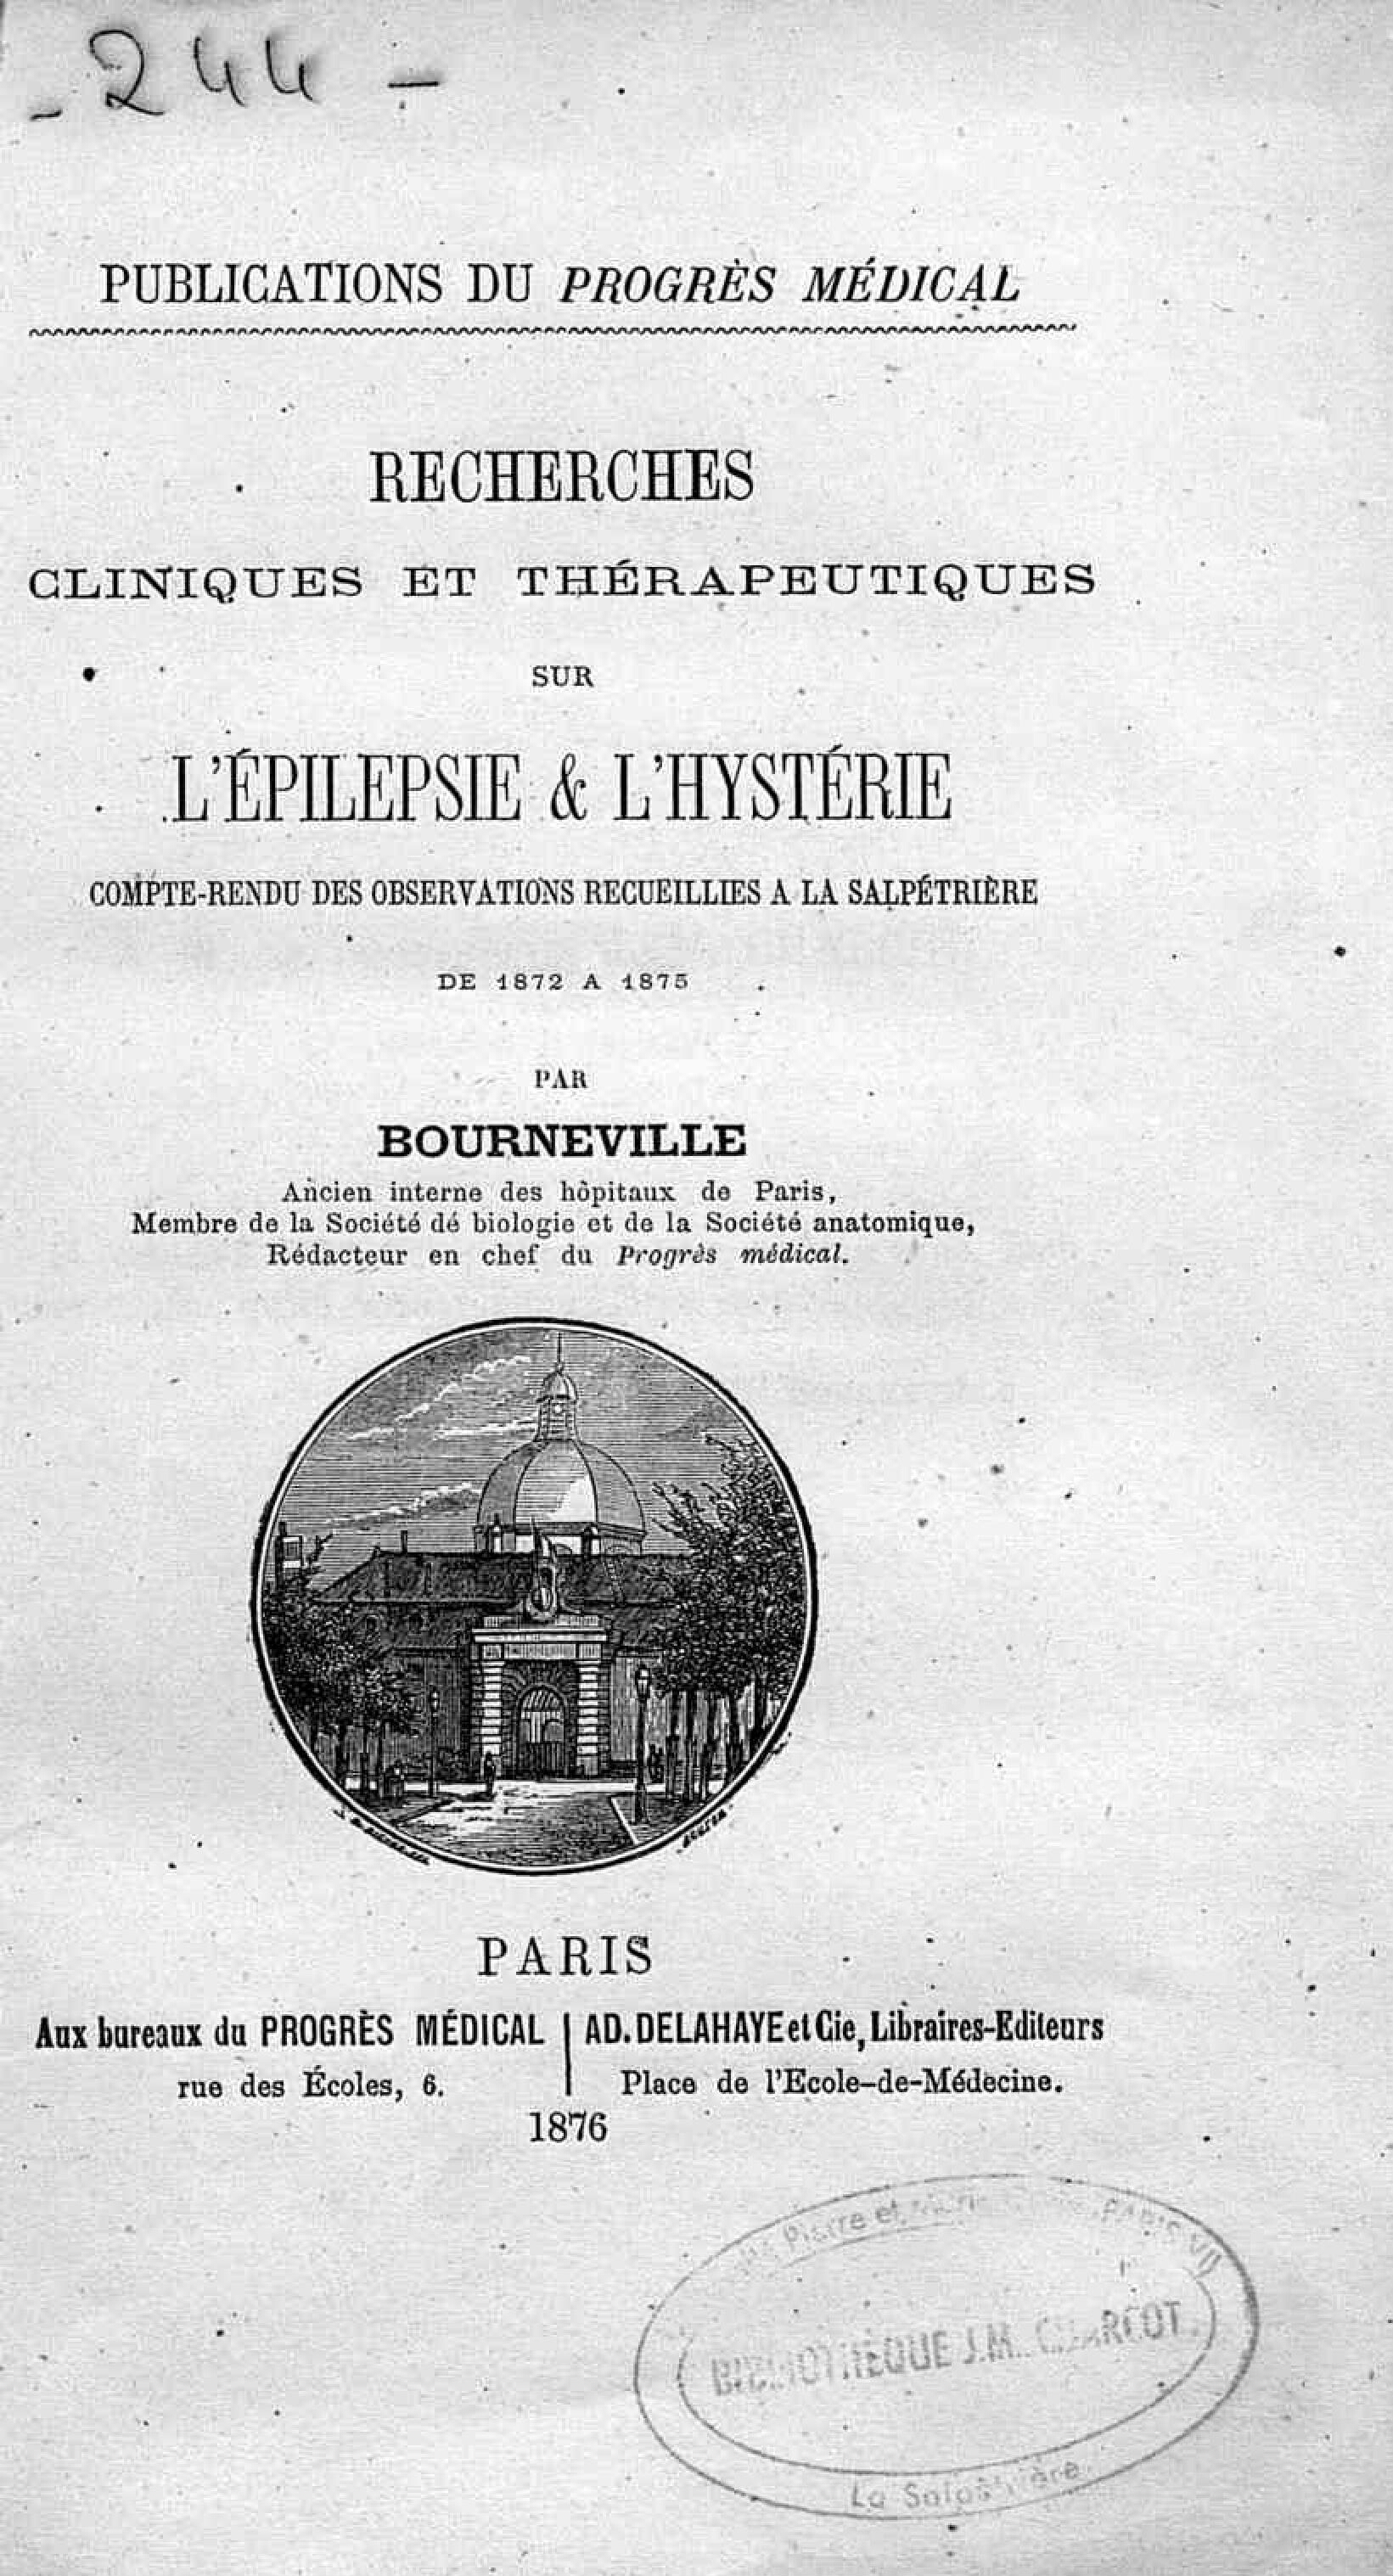
\includegraphics[height=6cm]{img/recherches_cliniques.jpg}
		\caption{Bourneville, D. M. (1876). \textit{Recherches cliniques et thérapeutiques sur l'épilepsie et l'hystérie : Compte-rendu des observations recueillies à la Salpêtrière de 1872 à 1875}. Bureaux du progrès médical (Paris). A. Delahaye (Paris)}
	\end{subfigure}\hfill
	\begin{subfigure}[t]{0.3\textwidth}
		\centering
		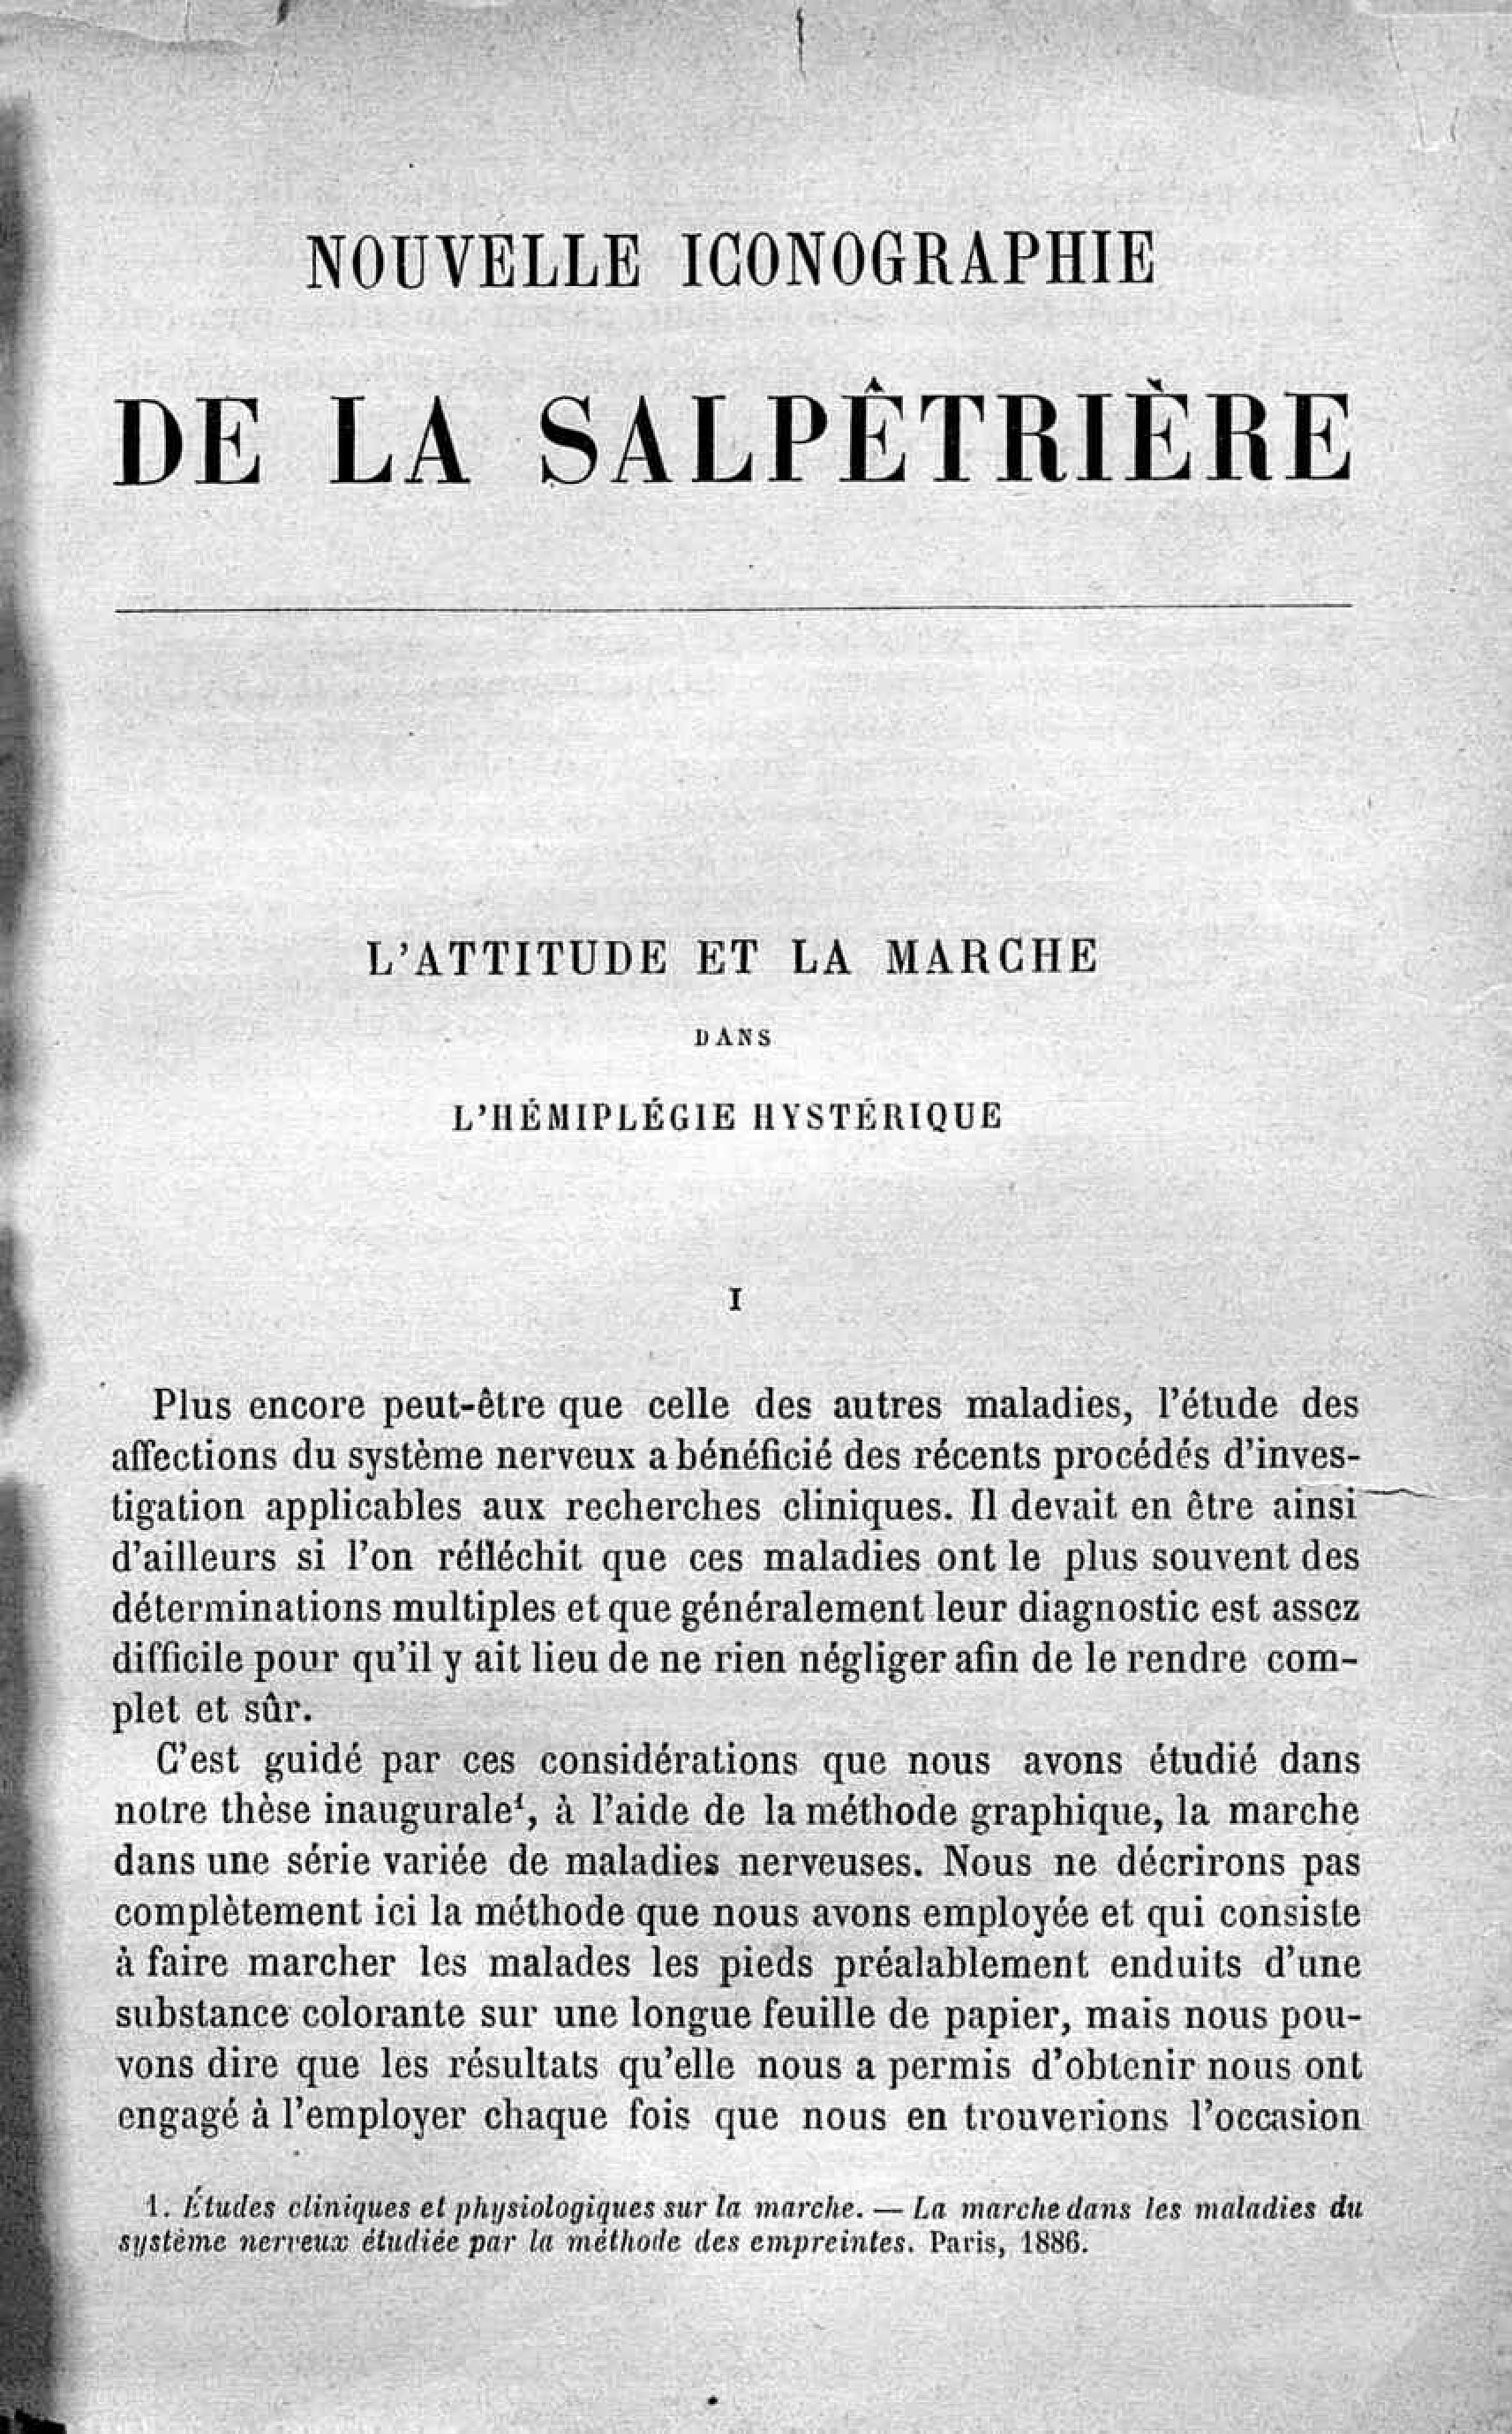
\includegraphics[height=6cm]{img/nouvelle_iconographie.jpg}
		\caption{de la Tourette, G. G. (1888). \textit{Nouvelle iconographie de la Salpêtrière [Tome 01] : clinique des maladies du système nerveux}. Lecrosnier et Babé (Paris).}
	\end{subfigure}
	
	\caption{Trois exemples de pages issues du corpus Autres.}
	\label{fig:autres_pages}
\end{figure}

Les figures \ref{fig:charcot_pages} et \ref{fig:autres_pages} donnent un aperçu visuel de notre corpus d'étude, avec quelques ouvrages représentatifs. Les documents sources peuvent être consultés dans le dépôt GitHub prévu à cet effet\footnote{\url{https://github.com/ljpetkovic/Charcot_circulations/tree/main/corpus}}. Le tableau \ref{tab:corpus_charcot} présente les documents constituant le corpus Charcot, classés selon l'ordre chronologique de leur publication.

\begingroup
\renewcommand{\arraystretch}{1.5}  % Add space between rows
\setstretch{0.9}                   % Shrink line spacing within cells

\footnotesize
\begin{longtable}
	{>{\raggedright\arraybackslash}p{0.20\textwidth}%
		>{\centering\arraybackslash}p{0.46\textwidth}%
		>{\raggedleft\arraybackslash}p{0.11\textwidth}%
		>{\raggedleft\arraybackslash}p{0.11\textwidth}}
	
	\toprule
	\textbf{Auteurs} & \textbf{Titre} & \textbf{Date} & \textbf{Tokens} \\
	\midrule
	\endfirsthead
	
	\toprule
	\textbf{Auteurs} & \textbf{Titre} & \textbf{Date} & \textbf{Tokens} \\
	\midrule
	\endhead
	
	\midrule \multicolumn{4}{r}{\textit{Suite à la page suivante}} \\
	\endfoot
	
	\bottomrule
	\endlastfoot
	
	\begin{minipage}[t]{\linewidth}\raggedright
		Richer, P.\\
		Charcot, J.-M.
	\end{minipage} &
	\begin{minipage}[t]{\linewidth}\raggedright
		\textit{Études cliniques sur l'hystéro-épilepsie ou\\
			Grande hystérie}
	\end{minipage} &
	1881 & 359 652 \\
	
	\addlinespace  % ← Adds space before the next row
	
	\begin{minipage}[t]{\linewidth}\raggedright
		Charcot, J.-M.\\
		Bourneville, D. M.
	\end{minipage} &
	\begin{minipage}[t]{\linewidth}\raggedright
		\textit{Archives de neurologie [Tome 01] : revue\\
			trimestrielle des maladies nerveuses et mentales}
	\end{minipage} &
	1881 & 302 295 \\
	
	\addlinespace  % ← Adds space before the next row
	
		
	\begin{minipage}[t]{\linewidth}\raggedright
		Charcot, J.-M.\\
		Bourneville, D. M.
	\end{minipage} &
	\begin{minipage}[t]{\linewidth}\raggedright
		\textit{Archives de neurologie [Tome 02, n° 05-06] : revue
			  trimestrielle des maladies nerveuses et mentales}
	\end{minipage} &
	1881 & 139 034 \\
	
	\addlinespace  % ← Adds space before the next row
	
	\begin{minipage}[t]{\linewidth}\raggedright
		Charcot, J.-M.\\
		Bourneville, D. M.
	\end{minipage} &
	\begin{minipage}[t]{\linewidth}\raggedright
		\textit{Archives de neurologie [Tome 03, n° 07-09] :\\
			 revue mensuelle des maladies nerveuses et mentales}
	\end{minipage} &
	1882 & 157 476 \\
	
		\addlinespace  % ← Adds space before the next row
	\begin{minipage}[t]{\linewidth}\raggedright
		Charcot, J.-M.\\
		Bourneville, D. M.
	\end{minipage} &
	\begin{minipage}[t]{\linewidth}\raggedright
		\textit{Archives de neurologie [Tome 04, n° 10-12] :\\
			revue mensuelle des maladies nerveuses et mentales}
	\end{minipage} &
	1882 & 169 894 \\
	
	\addlinespace  % ← Adds space before the next row
	
	\begin{minipage}[t]{\linewidth}\raggedright
		Charcot, J.-M.\\
		Bourneville, D. M.
	\end{minipage} &
	\begin{minipage}[t]{\linewidth}\raggedright
		\textit{Archives de neurologie [Tome 05, n° 13-15] :\\
			revue mensuelle des maladies nerveuses et mentales}
	\end{minipage} &
	1883 & 206 003 \\
	
			\addlinespace  % ← Adds space before the next row
	\begin{minipage}[t]{\linewidth}\raggedright
		Charcot, J.-M.\\
Bourneville, D. M.
	\end{minipage} &
	\begin{minipage}[t]{\linewidth}\raggedright
		\textit{Archives de neurologie [Tome 06, n° 16-18] :\\
			revue mensuelle des maladies nerveuses et mentales}
	\end{minipage} &
	1883 & 233 640 \\
	
	\addlinespace  % ← Adds space before the next row
	
	\begin{minipage}[t]{\linewidth}\raggedright
		Charcot, J.-M.\\
		Bourneville, D. M.
	\end{minipage} &
	\begin{minipage}[t]{\linewidth}\raggedright
		\textit{Archives de neurologie [Tome 07, n° 19-21] :\\
			revue mensuelle des maladies nerveuses et mentales}
	\end{minipage} &
	1884 & 183 645 \\
		\addlinespace  % ← Adds space before the next row
		
	\begin{minipage}[t]{\linewidth}\raggedright
		Charcot, J.-M.\\
	Bourneville, D. M.
	\end{minipage} &
	\begin{minipage}[t]{\linewidth}\raggedright
		\textit{Archives de neurologie [Tome 08, n° 22-24] :\\
			revue des maladies nerveuses et mentales}
	\end{minipage} &
	1884 & 187 544 \\
	
	\addlinespace  % ← Adds space before the next row
	
	\begin{minipage}[t]{\linewidth}\raggedright
		Charcot, J.-M.\\
		Bourneville, D. M.
	\end{minipage} &
	\begin{minipage}[t]{\linewidth}\raggedright
		\textit{Archives de neurologie [Tome 09, n° 25-27] :\\
			revue mensuelle des maladies nerveuses et mentales}
	\end{minipage} &
	1885 & 191 466 \\
	
		\addlinespace  % ← Adds space before the next row
	
	\begin{minipage}[t]{\linewidth}\raggedright
		Charcot, J.-M.\\
		Bourneville, D. M.
	\end{minipage} &
	\begin{minipage}[t]{\linewidth}\raggedright
		\textit{Archives de neurologie [Tome 10, n° 28-30] :\\
			revue des maladies nerveuses et mentales}
	\end{minipage} &
	1885 & 208 340 \\
	
			\addlinespace  % ← Adds space before the next row
	
	\begin{minipage}[t]{\linewidth}\raggedright
		Charcot, J.-M.\\
		Bourneville, D. M.
	\end{minipage} &
	\begin{minipage}[t]{\linewidth}\raggedright
		\textit{Archives de neurologie [Tome 11, n° 31-33] :\\
			revue mensuelle des maladies nerveuses et mentales}
	\end{minipage} &
	1886 & 197 029 \\
	
				\addlinespace  % ← Adds space before the next row
	
	\begin{minipage}[t]{\linewidth}\raggedright
		Charcot, J.-M.\\
		Bourneville, D. M.
	\end{minipage} &
	\begin{minipage}[t]{\linewidth}\raggedright
		\textit{Archives de neurologie [Tome 12, n° 34-36] :\\
			revue mensuelle des maladies nerveuses et mentales}
	\end{minipage} &
	1886 & 183 053 \\
	
					\addlinespace  % ← Adds space before the next row
	
	\begin{minipage}[t]{\linewidth}\raggedright
		Bourneville, D. M.\\
		Charcot, J.-M.
	\end{minipage} &
	\begin{minipage}[t]{\linewidth}\raggedright
		\textit{\OE{}uvres complètes de J. M. Charcot. Tome 2.\\
			Leçons sur les maladies du système nerveux.}
	\end{minipage} &
	1886 & 192 947 \\
	
						\addlinespace  % ← Adds space before the next row
	
	\begin{minipage}[t]{\linewidth}\raggedright
		Charcot, J.-M.\\
		Bourneville, D. M.
	\end{minipage} &
	\begin{minipage}[t]{\linewidth}\raggedright
		\textit{Archives de neurologie [Tome 13, n° 37-39] :\\
			revue mensuelle des maladies nerveuses et mentales}
	\end{minipage} &
	1887 & 214 235 \\
	
	
	\addlinespace  % ← Adds space before the next row
	
	\begin{minipage}[t]{\linewidth}\raggedright
		Charcot, J.-M.\\
		Bourneville, D. M.
	\end{minipage} &
	\begin{minipage}[t]{\linewidth}\raggedright
		\textit{Archives de neurologie [Tome 14, n° 40-42] :\\
			revue mensuelle des maladies nerveuses et mentales}
	\end{minipage} &
	1887 & 197 160 \\
	
		
	\addlinespace  % ← Adds space before the next row
	
	\begin{minipage}[t]{\linewidth}\raggedright
		Charcot, J.-M.\\
		Bourneville, D. M.
	\end{minipage} &
	\begin{minipage}[t]{\linewidth}\raggedright
		\textit{Archives de neurologie [Tome 15, n° 43-45] :\\
			revue mensuelle des maladies nerveuses et mentales}
	\end{minipage} &
	1888 & 210 025 \\
	
		\addlinespace  % ← Adds space before the next row
	
	\begin{minipage}[t]{\linewidth}\raggedright
		Charcot, J.-M.\\
		Bourneville, D. M.
	\end{minipage} &
	\begin{minipage}[t]{\linewidth}\raggedright
		\textit{Archives de neurologie [Tome 16, n° 46-48] :\\
			revue mensuelle des maladies nerveuses et mentales}
	\end{minipage} &
	1888 & 218 916 \\
	
			\addlinespace  % ← Adds space before the next row
	
	\begin{minipage}[t]{\linewidth}\raggedright
		Brissaud, É.\\
		Charcot, J.-M.\\
		Bourneville, D. M.
	\end{minipage} &
	\begin{minipage}[t]{\linewidth}\raggedright
		\textit{\OE{}uvres complètes de J. M. Charcot. Tome 5.\\
			Maladies des poumons et du système vasculaire.}
	\end{minipage} &
	1888 & 235 180 \\
	
				\addlinespace  % ← Adds space before the next row
	
	\begin{minipage}[t]{\linewidth}\raggedright
		Charcot, J.-M.\\
		Bourneville, D. M.
	\end{minipage} &
	\begin{minipage}[t]{\linewidth}\raggedright
		\textit{Archives de neurologie [Tome 17, n° 49-51] :\\
			revue mensuelle des maladies nerveuses et mentales}
	\end{minipage} &
	1889 & 212 629 \\
	
					\addlinespace  % ← Adds space before the next row
	
	\begin{minipage}[t]{\linewidth}\raggedright
		Charcot, J.-M.\\
		Bourneville, D. M.
	\end{minipage} &
	\begin{minipage}[t]{\linewidth}\raggedright
		\textit{Archives de neurologie [Tome 18, n° 52-54] :\\
			revue mensuelle des maladies nerveuses et mentales}
	\end{minipage} &
	1889 & 198 024 \\
						\addlinespace  % ← Adds space before the next row
	
	\begin{minipage}[t]{\linewidth}\raggedright
		Bourneville, D. M.\\
		Charcot, J.-M.
	\end{minipage} &
	\begin{minipage}[t]{\linewidth}\raggedright
		\textit{\OE{}uvres complètes de J. M. Charcot. Tome 8.\\
			Maladies infectieuses, affections de la peau,\\
			kystes hydatiques, estomac et rate, thérapeutique}
	\end{minipage} &
	1889 & 167 498 \\
	
							\addlinespace  % ← Adds space before the next row
	
	\begin{minipage}[t]{\linewidth}\raggedright
		Blin, E.\\
		Colin, H.\\
		Charcot, J.-M.\\
		Charcot, J.-B.
	\end{minipage} &
	\begin{minipage}[t]{\linewidth}\raggedright
		\textit{Leçons du Mardi à la Salpêtrière.\\
			Policlinique 1888-1889}
	\end{minipage} &
	1889 & 269 068 \\
	
					\addlinespace  % ← Adds space before the next row

\begin{minipage}[t]{\linewidth}\raggedright
	Charcot, J.-M.\\
	Bourneville, D. M.
\end{minipage} &
\begin{minipage}[t]{\linewidth}\raggedright
	\textit{Archives de neurologie [Tome 19, n° 55-57] :\\
		revue des maladies nerveuses et mentales}
\end{minipage} &
1890 & 178 499 \\

					\addlinespace  % ← Adds space before the next row

\begin{minipage}[t]{\linewidth}\raggedright
	Charcot, J.-M.\\
	Bourneville, D. M.
\end{minipage} &
\begin{minipage}[t]{\linewidth}\raggedright
	\textit{Archives de neurologie [Tome 20, n° 58-60] :\\
		revue mensuelle des maladies nerveuses et mentales}
\end{minipage} &
1890 & 201 754 \\

					\addlinespace  % ← Adds space before the next row

\begin{minipage}[t]{\linewidth}\raggedright
	Brissaud, É.\\
	Charcot, J.-M.\\
	Tourette, G. G. de la\\
	Babinski, J.\\
	Féré, C.\\
	Bourneville, D. M.\\
	Bernard, D.
\end{minipage} &

\begin{minipage}[t]{\linewidth}
%	\vspace*{0.9\baselineskip} % Ajuste ce facteur selon le nombre d'auteurs
	\raggedright
	\textit{\OE{}uvres complètes de J. M. Charcot. Tome 3.\\
		Leçons sur les maladies du système nerveux}
\end{minipage} &

1890 & 182 542 \\

	
						\addlinespace  % ← Adds space before the next row
	
	\begin{minipage}[t]{\linewidth}\raggedright
		Ball, B.\\
		Charcot, J.-M.\\
		Joffroy, A.\\
		Bourneville, D. M.
	\end{minipage} &
	\begin{minipage}[t]{\linewidth}\raggedright
		\textit{\OE{}uvres complètes de J. M. Charcot. Tome 7.\\
			Maladies des vieillards : goutte et rhumatisme}
	\end{minipage} &
	1890 & 224 619 \\
	
							\addlinespace  % ← Adds space before the next row
	
	\begin{minipage}[t]{\linewidth}\raggedright
		Bourneville, D. M.\\
		Charcot, J.-M.
	\end{minipage} &
	\begin{minipage}[t]{\linewidth}\raggedright
		\textit{\OE{}uvres complètes de J. M. Charcot. Tome 9.\\
			Hémorragie et ramollissement du cerveau, métallothérapie et hypnotisme, électrothérapie}
	\end{minipage} &
	1890 & 180 982 \\
	
								\addlinespace  % ← Adds space before the next row
	
	\begin{minipage}[t]{\linewidth}\raggedright
		Charcot, J.-M.\\
		Bourneville, D. M.
	\end{minipage} &
	\begin{minipage}[t]{\linewidth}\raggedright
		\textit{Archives de neurologie [Tome 21, n° 61-63] :\\
			revue mensuelle des maladies nerveuses et mentales}
	\end{minipage} &
	1891 & 216 741 \\
	
									\addlinespace  % ← Adds space before the next row
	
	\begin{minipage}[t]{\linewidth}\raggedright
		Charcot, J.-M.\\
		Bourneville, D. M.
	\end{minipage} &
	\begin{minipage}[t]{\linewidth}\raggedright
		\textit{Archives de neurologie [Tome 22, n° 64-66] :\\
			revue mensuelle des maladies nerveuses et mentales}
	\end{minipage} &
	1891 & 205 548 \\
	
		\addlinespace  % ← Adds space before the next row
	
	\begin{minipage}[t]{\linewidth}\raggedright
		Charcot, J.-M.\\
		Londe, A.\\
		Blocq, P.
	\end{minipage} &
	\begin{minipage}[t]{\linewidth}\raggedright
		\textit{Anatomie pathologique de la moëlle épinière :\\
			45 planches en héliogravure avec le texte explicatif}
	\end{minipage} &
	1891 & 15 066 \\
	
			\addlinespace  % ← Adds space before the next row
	
	\begin{minipage}[t]{\linewidth}\raggedright
		Brissaud, É.\\
		Charcot, J.-M.\\
		Sevestre, L. A.\\
		Bourneville, D. M.
	\end{minipage} &
	\begin{minipage}[t]{\linewidth}\raggedright
		\textit{\OE{}uvres complètes de J. M. Charcot.\\
			Leçons sur les maladies du foie et des reins. Tome 6}
	\end{minipage} &
	1891 & 159 395 \\
		
	\addlinespace  % ← Adds space before the next row
	
	\begin{minipage}[t]{\linewidth}\raggedright
		Charcot, J.-M.\\
		Bourneville, D. M.
	\end{minipage} &
	\begin{minipage}[t]{\linewidth}\raggedright
		\textit{Archives de neurologie [Tome 23, n° 67-69] :\\
			revue mensuelle des maladies nerveuses et mentales}
	\end{minipage} &
	1892 & 202 726 \\
	
		\addlinespace  % ← Adds space before the next row
	
	\begin{minipage}[t]{\linewidth}\raggedright
		Charcot, J.-M.\\
		Bourneville, D. M.
	\end{minipage} &
	\begin{minipage}[t]{\linewidth}\raggedright
		\textit{Archives de neurologie [Tome 24, n° 70-72] :\\
			revue mensuelle des maladies nerveuses et mentales}
	\end{minipage} &
	1892 & 253 978 \\
	
			\addlinespace  % ← Adds space before the next row
	
	\begin{minipage}[t]{\linewidth}\raggedright
		Bourneville, D. M.\\
		Charcot, J.-M.
	\end{minipage} &
	\begin{minipage}[t]{\linewidth}\raggedright
		\textit{\OE{}uvres complètes de J. M. Charcot. Tome 1.\\
			 Leçons sur les maladies du système nerveux}
	\end{minipage} &
	1892 & 193 105 \\
	
		
	\addlinespace  % ← Adds space before the next row
	
	\begin{minipage}[t]{\linewidth}\raggedright
		Guinon, G.\\
		Charcot, J.-M.
	\end{minipage} &
	\begin{minipage}[t]{\linewidth}\raggedright
		\textit{Clinique des maladies du système nerveux :
			leçons du professeur, mémoires, notes et observations :
			parus pendant les années 1889-90 et 1890-91. Tome 1}
	\end{minipage} &
	1892 & 162 512 \\
	
			\addlinespace  % ← Adds space before the next row
	
	\begin{minipage}[t]{\linewidth}\raggedright
		Charcot, J.-M.\\
		Bourneville, D. M.
	\end{minipage} &
	\begin{minipage}[t]{\linewidth}\raggedright
		\textit{Archives de neurologie [Tome 25, n° 73-76] :\\
			revue mensuelle des maladies nerveuses et mentales}
	\end{minipage} &
	1893 & 215 055 \\
	
				\addlinespace  % ← Adds space before the next row
	
	\begin{minipage}[t]{\linewidth}\raggedright
		Charcot, J.-M.\\
		Bourneville, D. M.
	\end{minipage} &
	\begin{minipage}[t]{\linewidth}\raggedright
		\textit{Archives de neurologie [Tome 26, n° 77-82] :\\
			revue des maladies nerveuses et mentales}
	\end{minipage} &
	1893 & 256 423 \\
	
					\addlinespace  % ← Adds space before the next row
	
	\begin{minipage}[t]{\linewidth}\raggedright
		Brissaud, É.\\
		Charcot, J.-M.\\
		Bourneville, D. M.
	\end{minipage} &
	\begin{minipage}[t]{\linewidth}\raggedright
		\textit{\OE{}uvres complètes de J. M. Charcot. Tome 4.\\
			Leçons sur les maladies du système nerveux}
	\end{minipage} &
	1893 & 139 088 \\
	
						\addlinespace  % ← Adds space before the next row
	
	\begin{minipage}[t]{\linewidth}\raggedright
		Guinon, G.\\
		Charcot, J.-M.\\
	\end{minipage} &
	\begin{minipage}[t]{\linewidth}\raggedright
		\textit{Clinique des maladies du système nerveux :
			leçons du professeur, mémoires, notes et observations :
			parus pendant les années 1889-90 et 1890-91. Tome 2}
	\end{minipage} &
	1893 & 191 190 \\
	
							\addlinespace  % ← Adds space before the next row
	
	\begin{minipage}[t]{\linewidth}\raggedright
		Charcot, J.-M.\\
		Bourneville, D. M.
	\end{minipage} &
	\begin{minipage}[t]{\linewidth}\raggedright
		\textit{Archives de neurologie [Tome 27, n° 83-88] :\\
			revue mensuelle des maladies nerveuses et mentales}
	\end{minipage} &
	1894 & 282 601 \\
	
								\addlinespace  % ← Adds space before the next row
	
	\begin{minipage}[t]{\linewidth}\raggedright
		Charcot, J.-M.\\
		Bourneville, D. M.
	\end{minipage} &
	\begin{minipage}[t]{\linewidth}\raggedright
		\textit{Archives de neurologie [Tome 28, n° 89-94] :\\
			revue mensuelle des maladies nerveuses et mentales}
	\end{minipage} &
	1894 & 264 965 \\
	
									\addlinespace  % ← Adds space before the next row
	
	\begin{minipage}[t]{\linewidth}\raggedright
		Charcot, J.-M.\\
		Bourneville, D. M.
	\end{minipage} &
	\begin{minipage}[t]{\linewidth}\raggedright
		\textit{Archives de neurologie [Tome 29, n° 95-100] :\\
			revue mensuelle des maladies nerveuses et mentales}
	\end{minipage} &
	1895 & 242 152 \\
	
										\addlinespace  % ← Adds space before the next row
	
	\begin{minipage}[t]{\linewidth}\raggedright
		Charcot, J.-M.\\
		Bourneville, D. M.
	\end{minipage} &
	\begin{minipage}[t]{\linewidth}\raggedright
		\textit{Archives de neurologie [Tome 30, n° 101-106] :\\
			revue mensuelle des maladies nerveuses et mentales}
	\end{minipage} &
	1895 & 241 618 \\
	
											\addlinespace  % ← Adds space before the next row
	
	\begin{minipage}[t]{\linewidth}\raggedright
		Charcot, J.-M.\\
		Bourneville, D. M.
	\end{minipage} &
	\begin{minipage}[t]{\linewidth}\raggedright
		\textit{Archives de neurologie [2\ieme{} série, tome 01, n° 01-06] :\\
			revue mensuelle des maladies nerveuses et mentales}
	\end{minipage} &
	1896 & 240 449 \\
	
												\addlinespace  % ← Adds space before the next row
	
	\begin{minipage}[t]{\linewidth}\raggedright
		Charcot, J.-M.\\
		Bourneville, D. M.
	\end{minipage} &
	\begin{minipage}[t]{\linewidth}\raggedright
		\textit{Archives de neurologie [2\ieme{} série, tome 02, n° 07-12] :\\
			revue mensuelle des maladies nerveuses et mentales}
	\end{minipage} &
	1896 & 238 233 \\
	
												\addlinespace  % ← Adds space before the next row
	
	\begin{minipage}[t]{\linewidth}\raggedright
		Charcot, J.-M.\\
		Bourneville, D. M.
	\end{minipage} &
	\begin{minipage}[t]{\linewidth}\raggedright
		\textit{Archives de neurologie [2\ieme{} série, tome 03, n° 13-18] :\\
			revue mensuelle des maladies nerveuses et mentales}
	\end{minipage} &
	1897 & 242 603 \\
	
													\addlinespace  % ← Adds space before the next row
	
	\begin{minipage}[t]{\linewidth}\raggedright
		Charcot, J.-M.\\
		Bourneville, D. M.
	\end{minipage} &
	\begin{minipage}[t]{\linewidth}\raggedright
		\textit{Archives de neurologie [2\ieme{} série, tome 04, n° 19-24] :\\
			revue mensuelle des maladies nerveuses et mentales}
	\end{minipage} &
	1897 & 260 016 \\
	
	\addlinespace  % ← Adds space before the next row
	
	\begin{minipage}[t]{\linewidth}\raggedright
		Charcot, J.-M.\\
		Bourneville, D. M.
	\end{minipage} &
	\begin{minipage}[t]{\linewidth}\raggedright
		\textit{Archives de neurologie [2\ieme{} série, tome 05, n° 25-30] :\\
			revue mensuelle des maladies nerveuses et mentales}
	\end{minipage} &
	1898 & 254 523 \\
	
		\addlinespace  % ← Adds space before the next row
	
	\begin{minipage}[t]{\linewidth}\raggedright
		Charcot, J.-M.\\
		Bourneville, D. M.
	\end{minipage} &
	\begin{minipage}[t]{\linewidth}\raggedright
		\textit{Archives de neurologie [2\ieme{} série, tome 06, n° 31-36] :\\
			revue mensuelle des maladies nerveuses et mentales}
	\end{minipage} &
	1898 & 249 002 \\
	
			\addlinespace  % ← Adds space before the next row
	
	\begin{minipage}[t]{\linewidth}\raggedright
		Charcot, J.-M.\\
		Bourneville, D. M.
	\end{minipage} &
	\begin{minipage}[t]{\linewidth}\raggedright
		\textit{Archives de neurologie [2\ieme{} série, tome 07, n° 37-42] :\\
			revue mensuelle des maladies nerveuses et mentales}
	\end{minipage} &
	1899 & 245 271 \\
	
	\addlinespace  % ← Adds space before the next row
	
	\begin{minipage}[t]{\linewidth}\raggedright
		Charcot, J.-M.\\
		Bourneville, D. M.
	\end{minipage} &
	\begin{minipage}[t]{\linewidth}\raggedright
		\textit{Archives de neurologie [2\ieme{} série, tome 08, n° 43-48] :\\
			revue mensuelle des maladies nerveuses et mentales}
	\end{minipage} &
	1899 & 261 298 \\
	
	\addlinespace  % ← Adds space before the next row
	
	\begin{minipage}[t]{\linewidth}\raggedright
		Charcot, J.-M.\\
		Bourneville, D. M.
	\end{minipage} &
	\begin{minipage}[t]{\linewidth}\raggedright
		\textit{Archives de neurologie [2\ieme{} série, tome 09, n° 49-54] :\\
			revue mensuelle des maladies nerveuses et mentales}
	\end{minipage} &
	1900 & 268 418 \\

	\addlinespace  % ← Adds space before the next row
	
	\begin{minipage}[t]{\linewidth}\raggedright
		Charcot, J.-M.\\
		Bourneville, D. M.
	\end{minipage} &
	\begin{minipage}[t]{\linewidth}\raggedright
		\textit{Archives de neurologie [2\ieme{} série, tome 10, n° 55-60] :\\
			revue mensuelle des maladies nerveuses et mentales}
	\end{minipage} &
	1900 & 251 199 \\
	
	\addlinespace  % ← Adds space before the next row
	
	\begin{minipage}[t]{\linewidth}\raggedright
		Charcot, J.-M.\\
		Bourneville, D. M.
	\end{minipage} &
	\begin{minipage}[t]{\linewidth}\raggedright
		\textit{Archives de neurologie [2\ieme{} série, tome 11, n° 61-66] :\\
			revue mensuelle des maladies nerveuses et mentales}
	\end{minipage} &
	1901 & 265 314 \\
		
	\addlinespace  % ← Adds space before the next row
	
	\begin{minipage}[t]{\linewidth}\raggedright
		Charcot, J.-M.\\
		Bourneville, D. M.
	\end{minipage} &
	\begin{minipage}[t]{\linewidth}\raggedright
		\textit{Archives de neurologie [2\ieme{} série, tome 12, n° 67-72] :\\
			revue mensuelle des maladies nerveuses et mentales}
	\end{minipage} &
	1901 & 250 842 \\
	
		\addlinespace  % ← Adds space before the next row
	
	\begin{minipage}[t]{\linewidth}\raggedright
		Charcot, J.-M.\\
		Bourneville, D. M.
	\end{minipage} &
	\begin{minipage}[t]{\linewidth}\raggedright
		\textit{Archives de neurologie [2\ieme{} série, tome 13, n° 73-78] :\\
			revue mensuelle des maladies nerveuses et mentales}
	\end{minipage} &
	1902 & 253 568 \\
	
		\addlinespace  % ← Adds space before the next row

	\begin{minipage}[t]{\linewidth}\raggedright
		Charcot, J.-M.\\
		Bourneville, D. M.
	\end{minipage} &
	\begin{minipage}[t]{\linewidth}\raggedright
		\textit{Archives de neurologie [2\ieme{} série, tome 14, n° 79-84] :\\
			revue mensuelle des maladies nerveuses et mentales}
	\end{minipage} &
	1902 & 247 303 \\
	
		
	\addlinespace  % ← Adds space before the next row
	
	\begin{minipage}[t]{\linewidth}\raggedright
		Charcot, J.-M.\\
		Bourneville, D. M.
	\end{minipage} &
	\begin{minipage}[t]{\linewidth}\raggedright
		\textit{Archives de neurologie [2\ieme{} série, tome 15, n° 85-90] :\\
			revue mensuelle des maladies nerveuses et mentales}
	\end{minipage} &
	1903 & 282 033 \\
	
		\addlinespace  % ← Adds space before the next row
	
	\begin{minipage}[t]{\linewidth}\raggedright
		Charcot, J.-M.\\
		Bourneville, D. M.
	\end{minipage} &
	\begin{minipage}[t]{\linewidth}\raggedright
		\textit{Archives de neurologie [2\ieme{} série, tome 16, n° 91-96] :\\
			revue mensuelle des maladies nerveuses et mentales}
	\end{minipage} &
	1903 & 254 397 \\
	
	\addlinespace  % ← Adds space before the next row
	
	\begin{minipage}[t]{\linewidth}\raggedright
		Charcot, J.-M.\\
		Bourneville, D. M.
	\end{minipage} &
	\begin{minipage}[t]{\linewidth}\raggedright
		\textit{Archives de neurologie [2\ieme{} série, tome 17, n° 97-102] :\\
			revue mensuelle des maladies nerveuses et mentales}
	\end{minipage} &
	1904 & 258 376 \\
	
		\addlinespace  % ← Adds space before the next row
	
	\begin{minipage}[t]{\linewidth}\raggedright
		Charcot, J.-M.\\
		Bourneville, D. M.
	\end{minipage} &
	\begin{minipage}[t]{\linewidth}\raggedright
		\textit{Archives de neurologie [2\ieme{} série, tome 18, n° 103-108] :\\
			revue mensuelle des maladies nerveuses et mentales}
	\end{minipage} &
	1904 & 245 612 \\
	
			\addlinespace  % ← Adds space before the next row
	
	\begin{minipage}[t]{\linewidth}\raggedright
		Charcot, J.-M.\\
		Bourneville, D. M.
	\end{minipage} &
	\begin{minipage}[t]{\linewidth}\raggedright
		\textit{Archives de neurologie [2\ieme{} série, tome 19, n° 109-114] :\\
			revue mensuelle des maladies nerveuses et mentales}
	\end{minipage} &
	1905 & 231 985 \\
	
			\addlinespace  % ← Adds space before the next row
	
	\begin{minipage}[t]{\linewidth}\raggedright
		Charcot, J.-M.\\
		Bourneville, D. M.
	\end{minipage} &
	\begin{minipage}[t]{\linewidth}\raggedright
		\textit{Archives de neurologie [2\ieme{} série, tome 20, n° 115-120] :\\
			revue mensuelle des maladies nerveuses et mentales}
	\end{minipage} &
	1905 & 237 686 \\
	
				\addlinespace  % ← Adds space before the next row
	
	\begin{minipage}[t]{\linewidth}\raggedright
		Charcot, J.-M.\\
		Bourneville, D. M.
	\end{minipage} &
	\begin{minipage}[t]{\linewidth}\raggedright
		\textit{Archives de neurologie [2\ieme{} série, tome 21, n° 121-126] :\\
			revue mensuelle des maladies nerveuses et mentales}
	\end{minipage} &
	1906 & 228 892 \\
	
					\addlinespace  % ← Adds space before the next row
	
	\begin{minipage}[t]{\linewidth}\raggedright
		Charcot, J.-M.\\
		Bourneville, D. M.
	\end{minipage} &
	\begin{minipage}[t]{\linewidth}\raggedright
		\textit{Archives de neurologie [2\ieme{} série, tome 22, n° 127-132] :\\
			revue mensuelle des maladies nerveuses et mentales}
	\end{minipage} &
	1906 & 217 906 \\
	
						\addlinespace  % ← Adds space before the next row
	
	\begin{minipage}[t]{\linewidth}\raggedright
		Charcot, J.-M.\\
		Bourneville, D. M.
	\end{minipage} &
	\begin{minipage}[t]{\linewidth}\raggedright
		\textit{Archives de neurologie [3\ieme{} série, tome 01, n° 01-06] :\\
			revue mensuelle des maladies nerveuses et mentales}
	\end{minipage} &
	1906 & 252 367 \\
	
							\addlinespace  % ← Adds space before the next row
	
	\begin{minipage}[t]{\linewidth}\raggedright
		Charcot, J.-M.\\
		Bourneville, D. M.
	\end{minipage} &
	\begin{minipage}[t]{\linewidth}\raggedright
		\textit{Archives de neurologie [3\ieme{} série, tome 02, n° 07-12] :\\
			revue mensuelle des maladies nerveuses et mentales}
	\end{minipage} &
	1907 & 243 008 \\
	
	\caption{Description du corpus Charcot.} \label{tab:corpus_charcot}
\end{longtable}
\normalsize
\endgroup




Les documents constituant le corpus Autres sont exposés dans le tableau \ref{tab:corpus_autres} ci-dessous :


\begingroup
\renewcommand{\arraystretch}{1.5}  % Add space between rows
\setstretch{0.9}                   % Shrink line spacing within cells

\footnotesize
\begin{longtable}
	{>{\raggedright\arraybackslash}p{0.20\textwidth}%
		>{\centering\arraybackslash}p{0.50\textwidth}%
		>{\raggedleft\arraybackslash}p{0.11\textwidth}%
		>{\raggedleft\arraybackslash}p{0.11\textwidth}}
	
	\toprule
	\textbf{Auteurs} & \textbf{Titre} & \textbf{Date} & \textbf{Tokens} \\
	\midrule
	\endfirsthead
	
	\toprule
	\textbf{Auteurs} & \textbf{Titre} & \textbf{Date} & \textbf{Tokens} \\
	\midrule
	\endhead
	
	\midrule \multicolumn{4}{r}{\textit{Suite à la page suivante}} \\
	\endfoot
	
	\bottomrule
	\endlastfoot
	
	\begin{minipage}[t]{\linewidth}\raggedright
	Desmoulin, A.\\
	Magendie, F.
	\end{minipage} &
	\begin{minipage}[t]{\linewidth}\raggedright
		\textit{Anatomie des systèmes nerveux des animaux à vertebres,\\
		appliquée à la physiologie et à la zoologie : Atlas}
	\end{minipage} &
	1825 & 5 932 \\
	
	\addlinespace  % ← Adds space before the next row
	
		\begin{minipage}[t]{\linewidth}\raggedright
		Cruveilhier, J.\\
		Chazal, A.
	\end{minipage} &
	\begin{minipage}[t]{\linewidth}\raggedright
		\textit{Anatomie pathologique du corps humain : ou descriptions 
			avec figures lithographiées et coloriées, des diverses altérations morbides dont le corps humain est susceptible. Tome premier}
	\end{minipage} &
	1829 & 397 308 \\
	
	\addlinespace  % ← Adds space before the next row
	
			\begin{minipage}[t]{\linewidth}\raggedright
		Cruveilhier, J.\\
		Chazal, A.
	\end{minipage} &
	\begin{minipage}[t]{\linewidth}\raggedright
		\textit{Anatomie pathologique du corps humain : ou descriptions 
			avec figures lithographiées et coloriées, des diverses altérations morbides dont le corps humain est susceptible. Tome second}
	\end{minipage} &
	1829 & 510 337 \\
	
	\addlinespace  % ← Adds space before the next row
	
				\begin{minipage}[t]{\linewidth}\raggedright
		Chazal, A.\\
		Leuret, F.\\
		Oudet\\
		Trélat, U.\\
		Gratiolet, P.-L.
	\end{minipage} &
	\begin{minipage}[t]{\linewidth}\raggedright
		\textit{Anatomie comparée du système nerveux considéré dans ses rapports avec l'intelligence. Tome premier}
	\end{minipage} &
	1839 & 224 750 \\
	
	\addlinespace  % ← Adds space before the next row
	
	\begin{minipage}[t]{\linewidth}\raggedright
	Chazal, A.\\
	Leuret, F.\\
	Oudet\\
	Trélat, U.\\
	Gratiolet, P.-L.
\end{minipage} &
\begin{minipage}[t]{\linewidth}\raggedright
	\textit{Anatomie comparée du système nerveux considéré dans ses rapports avec l'intelligence. Tome second}
\end{minipage} &
1839 & 252 747 \\

\addlinespace  % ← Adds space before the next row

	\begin{minipage}[t]{\linewidth}\raggedright
	Foville, A. L.\\
	Bion, F.\\
	Beau, É.
\end{minipage} &
\begin{minipage}[t]{\linewidth}\raggedright
	\textit{Traité complet de l'anatomie, de la physiologie et de la pathologie du système nerveux cérébro-spinal. Première partie. Anatomie}
\end{minipage} &
1844 & 14 447 \\

\addlinespace  % ← Adds space before the next row

	\begin{minipage}[t]{\linewidth}\raggedright
	Société de magnétiseurs et de médecins
\end{minipage} &
\begin{minipage}[t]{\linewidth}\raggedright
	\textit{Journal du magnétisme [Tome I]}
\end{minipage} &
1845 & 176 491 \\

\addlinespace  % ← Adds space before the next row

	\begin{minipage}[t]{\linewidth}\raggedright
	Société de magnétiseurs et de médecins
\end{minipage} &
\begin{minipage}[t]{\linewidth}\raggedright
	\textit{Journal du magnétisme [Tome II et III]}
\end{minipage} &
1846 & 214 366 \\

\addlinespace  % ← Adds space before the next row

	\begin{minipage}[t]{\linewidth}\raggedright
	Société de magnétiseurs et de médecins
\end{minipage} &
\begin{minipage}[t]{\linewidth}\raggedright
	\textit{Journal du magnétisme [Tome IV et V]}
\end{minipage} &
1847 & 259 900 \\

\addlinespace  % ← Adds space before the next row

	\begin{minipage}[t]{\linewidth}\raggedright
	Société de magnétiseurs et de médecins
\end{minipage} &
\begin{minipage}[t]{\linewidth}\raggedright
	\textit{Journal du magnétisme [Tome VI et VII]}
\end{minipage} &
1848 & 244 182 \\

\addlinespace  % ← Adds space before the next row

	\begin{minipage}[t]{\linewidth}\raggedright
	Société de magnétiseurs et de médecins
\end{minipage} &
\begin{minipage}[t]{\linewidth}\raggedright
	\textit{Journal du magnétisme [Tome VIII]}
\end{minipage} &
1849 & 209 036 \\

\addlinespace  % ← Adds space before the next row

	\begin{minipage}[t]{\linewidth}\raggedright
	Société de magnétiseurs et de médecins
\end{minipage} &
\begin{minipage}[t]{\linewidth}\raggedright
	\textit{Journal du magnétisme [Tome IX]}
\end{minipage} &
1850 & 168 735 \\

\addlinespace  % ← Adds space before the next row

	\begin{minipage}[t]{\linewidth}\raggedright
	Société de magnétiseurs et de médecins
\end{minipage} &
\begin{minipage}[t]{\linewidth}\raggedright
	\textit{Journal du magnétisme [Tome X]}
\end{minipage} &
1851 & 254 771 \\

\addlinespace  % ← Adds space before the next row

	\begin{minipage}[t]{\linewidth}\raggedright
	Société de magnétiseurs et de médecins
\end{minipage} &
\begin{minipage}[t]{\linewidth}\raggedright
	\textit{Journal du magnétisme [Tome XI]}
\end{minipage} &
1852 & 18 656 \\

\addlinespace  % ← Adds space before the next row

	\begin{minipage}[t]{\linewidth}\raggedright
	Société de magnétiseurs et de médecins
\end{minipage} &
\begin{minipage}[t]{\linewidth}\raggedright
	\textit{Journal du magnétisme [Tome XII]}
\end{minipage} &
1853 & 263 294 \\

\addlinespace  % ← Adds space before the next row

	\begin{minipage}[t]{\linewidth}\raggedright
	Société de magnétiseurs et de médecins
\end{minipage} &
\begin{minipage}[t]{\linewidth}\raggedright
	\textit{Journal du magnétisme [Tome XIII]}
\end{minipage} &
1854 & 304 922 \\

\addlinespace  % ← Adds space before the next row

	\begin{minipage}[t]{\linewidth}\raggedright
	Gratiolet, P.-L.
\end{minipage} &
\begin{minipage}[t]{\linewidth}\raggedright
	\textit{Mémoire sur les plis cérébraux de l'homme et des primatès]}
\end{minipage} &
1854 & 51 715\\

\addlinespace  % ← Adds space before the next row

	\begin{minipage}[t]{\linewidth}\raggedright
	Gratiolet, P.-L.
\end{minipage} &
\begin{minipage}[t]{\linewidth}\raggedright
	\textit{Mémoire sur les plis cérébraux de l'homme et des primatès. Atlas]}
\end{minipage} &
1854 & 1 844\\

\addlinespace  % ← Adds space before the next row
	
		\begin{minipage}[t]{\linewidth}\raggedright
		Société de magnétiseurs et de médecins
	\end{minipage} &
	\begin{minipage}[t]{\linewidth}\raggedright
		\textit{Journal du magnétisme [Tome XIV]}
	\end{minipage} &
	1855 & 262 158 \\
	
	\addlinespace  % ← Adds space before the next row
	
			\begin{minipage}[t]{\linewidth}\raggedright
		Société de magnétiseurs et de médecins
	\end{minipage} &
	\begin{minipage}[t]{\linewidth}\raggedright
		\textit{Journal du magnétisme [Tome XV]}
	\end{minipage} &
	1856 & 263 290 \\
	
	\addlinespace  % ← Adds space before the next row
	
			\begin{minipage}[t]{\linewidth}\raggedright
		Société de magnétiseurs et de médecins
	\end{minipage} &
	\begin{minipage}[t]{\linewidth}\raggedright
		\textit{Journal du magnétisme [Tome XVI]}
	\end{minipage} &
	1857 & 261 600 \\
	
	\addlinespace  % ← Adds space before the next row
	
		
	\begin{minipage}[t]{\linewidth}\raggedright
		Chazal, A.\\
		Leuret, F.\\
		Oudet\\
		Trélat, U.\\
		Gratiolet, P.-L.
	\end{minipage} &
	\begin{minipage}[t]{\linewidth}\raggedright
		\textit{Anatomie comparée du système nerveux considéré dans ses rapports avec l'intelligence. Atlas}
	\end{minipage} &
	1857 & 26 070 \\
	
	\addlinespace  % ← Adds space before the next row
	
		\begin{minipage}[t]{\linewidth}\raggedright
			Bouvier, S. H. V.
	\end{minipage} &
	\begin{minipage}[t]{\linewidth}\raggedright
		\textit{Leçons cliniques sur les maladies chroniques de l'appareil locomoteur : professées à l'Hôpital des enfants malades pendant les années 1855, 1856, 1857}
	\end{minipage} &
	1858 & 234 727 \\
	
	\addlinespace  % ← Adds space before the next row

	\begin{minipage}[t]{\linewidth}\raggedright
		Bouvier, S. H. V.
	\end{minipage} &
	\begin{minipage}[t]{\linewidth}\raggedright
		\textit{Leçons cliniques sur les maladies chroniques de l'appareil locomoteur : professées à l'Hôpital des enfants malades pendant les années 1855, 1856, 1857. Déviations de la colonne vertébrale. Atlas de XX planches}
	\end{minipage} &
	1858 & 18 328 \\
	
	\addlinespace  % ← Adds space before the next row	
	\begin{minipage}[t]{\linewidth}\raggedright
		Société de magnétiseurs et de médecins
	\end{minipage} &
	\begin{minipage}[t]{\linewidth}\raggedright
		\textit{Journal du magnétisme [Tome XVIII]}
	\end{minipage} &
	1859 & 270 098 \\
	
	\addlinespace  % ← Adds space before the next row
	
		\begin{minipage}[t]{\linewidth}\raggedright
		Société de magnétiseurs et de médecins
	\end{minipage} &
	\begin{minipage}[t]{\linewidth}\raggedright
		\textit{Journal du magnétisme [Tome XIX]}
	\end{minipage} &
	1860 & 262 013 \\
	
	\addlinespace  % ← Adds space before the next row
	
		
	\begin{minipage}[t]{\linewidth}\raggedright
		Société de magnétiseurs et de médecins
	\end{minipage} &
	\begin{minipage}[t]{\linewidth}\raggedright
		\textit{Journal du magnétisme [Tome XX]}
	\end{minipage} &
	1861 & 182 523 \\
	
	\addlinespace  % ← Adds space before the next row
	
		\begin{minipage}[t]{\linewidth}\raggedright
		Duchenne, G.-B.
	\end{minipage} &
	\begin{minipage}[t]{\linewidth}\raggedright
		\textit{Mécanisme de la physionomie humaine : ou analyse électro-physiologique de l'expression des passions}
	\end{minipage} &
	1862 & 69 422 \\
	
	\addlinespace  % ← Adds space before the next row
	
			\begin{minipage}[t]{\linewidth}\raggedright
		Bourgery, J.-M.\\
		Jacob, N.-H.\\
		Bernard, C.
	\end{minipage} &
	\begin{minipage}[t]{\linewidth}\raggedright
		\textit{Traité complet de l'anatomie de l'homme comprenant l'anatomie chirurgicale et la médecine opératoire. Tome sixième. Anatomie chirurgicale et médecine opératoire. Première partie}
	\end{minipage} &
	1866 & 421 722 \\
	
	\addlinespace  % ← Adds space before the next row
	
	\begin{minipage}[t]{\linewidth}\raggedright
		Bourgery, J.-M.\\
		Jacob, N.-H.\\
		Bernard, C.
	\end{minipage} &
	\begin{minipage}[t]{\linewidth}\raggedright
		\textit{Traité complet de l'anatomie de l'homme comprenant l'anatomie chirurgicale et la médecine opératoire. Tome septième. Anatomie chirurgicale et médecine opératoire. Deuxième partie}
	\end{minipage} &
	1866 & 641 189 \\
	
	\addlinespace  % ← Adds space before the next row
	
		\begin{minipage}[t]{\linewidth}\raggedright
		Bourgery, J.-M.\\
		Jacob, N.-H.\\
		Bernard, C.
	\end{minipage} &
	\begin{minipage}[t]{\linewidth}\raggedright
		\textit{Traité complet de l'anatomie de l'homme comprenant l'anatomie chirurgicale et la médecine opératoire. Anatomie chirurgicale et médecine opératoire. Suppléments}
	\end{minipage} &
	1867 & 165 261 \\
	
	\addlinespace  % ← Adds space before the next row
	
			\begin{minipage}[t]{\linewidth}\raggedright
		Bourneville, D. M.\\
		Montméja, A. de
	\end{minipage} &
	\begin{minipage}[t]{\linewidth}\raggedright
		\textit{Revue photographique des hôpitaux de Paris. 1\ieme{} année}
	\end{minipage} &
	1869 & 77 945 \\
	
	\addlinespace  % ← Adds space before the next row
	
				\begin{minipage}[t]{\linewidth}\raggedright
		Bourneville, D. M.\\
		Montméja, A. de
	\end{minipage} &
	\begin{minipage}[t]{\linewidth}\raggedright
		\textit{Revue photographique des hôpitaux de Paris. 2\ieme{} année}
	\end{minipage} &
	1870 & 114 586 \\
	
	\addlinespace  % ← Adds space before the next row
	
		\begin{minipage}[t]{\linewidth}\raggedright
		Bourneville, D. M.\\
		Montméja, A. de
	\end{minipage} &
	\begin{minipage}[t]{\linewidth}\raggedright
		\textit{Revue photographique des hôpitaux de Paris. 3\ieme{} année}
	\end{minipage} &
	1871 & 149 848 \\
	
	\addlinespace  % ← Adds space before the next row
	
			\begin{minipage}[t]{\linewidth}\raggedright
		Bourneville, D. M.\\
		Montméja, A. de
	\end{minipage} &
	\begin{minipage}[t]{\linewidth}\raggedright
		\textit{Revue photographique des hôpitaux de Paris. 4\ieme{} année}
	\end{minipage} &
	1872 & 200 205 \\
	
	\addlinespace  % ← Adds space before the next row
	
				\begin{minipage}[t]{\linewidth}\raggedright
		Regnard, P.\\
		Bourneville, D. M.
	\end{minipage} &
	\begin{minipage}[t]{\linewidth}\raggedright
		\textit{Iconographie photographique de la Salpêtrière. Service de M. Charcot, 1875}
	\end{minipage} &
	1875 & 66 \\
	
	\addlinespace  % ← Adds space before the next row
	
			\begin{minipage}[t]{\linewidth}\raggedright
		Bourneville, D. M.
	\end{minipage} &
	\begin{minipage}[t]{\linewidth}\raggedright
		\textit{Recherches cliniques et thérapeutiques sur l'épilepsie et l'hystérie : Compte-rendu des observations recueillies à la Salpêtrière de 1872 à 1875}
	\end{minipage} &
	1876 & 74 582 \\
	
	\addlinespace  % ← Adds space before the next row
	
		\begin{minipage}[t]{\linewidth}\raggedright
		Regnard, P.\\
		Bourneville, D. M.
	\end{minipage} &
	\begin{minipage}[t]{\linewidth}\raggedright
		\textit{Iconographie photographique de la Salpêtrière. Service de M. Charcot, 1877}
	\end{minipage} &
	1877 & 60 543 \\
	
	\addlinespace  % ← Adds space before the next row
	
			\begin{minipage}[t]{\linewidth}\raggedright
		Regnard, P.\\
		Bourneville, D. M.
	\end{minipage} &
	\begin{minipage}[t]{\linewidth}\raggedright
		\textit{Iconographie photographique de la Salpêtrière. Service de M. Charcot, 1878}
	\end{minipage} &
	1878 & 84 675 \\
	
	\addlinespace  % ← Adds space before the next row
	
	\begin{minipage}[t]{\linewidth}\raggedright
		Regnard, P.\\
		Bourneville, D. M.
	\end{minipage} &
	\begin{minipage}[t]{\linewidth}\raggedright
		\textit{Iconographie photographique de la Salpêtrière. Service de M. Charcot, 1880}
	\end{minipage} &
	1880 & 83 211 \\
	
	\addlinespace  % ← Adds space before the next row
	
		\begin{minipage}[t]{\linewidth}\raggedright
		Bourneville, D. M.\\
		Service des épileptiques et des enfants idiots et arriérés de Bicêtre
	\end{minipage} &
	\begin{minipage}[t]{\linewidth}\raggedright
		\textit{Recherches cliniques et thérapeutiques sur l'épilepsie, l'hystérie et l'idiotie : Compte-rendu du service des épileptiques et des enfants idiots et arriérés de Bicêtre pendant l'année 1880}
	\end{minipage} &
	1881 & 48 983 \\
	
	\addlinespace  % ← Adds space before the next row
	
			\begin{minipage}[t]{\linewidth}\raggedright
		Bourneville, D. M.\\
		Service des épileptiques et des enfants idiots et arriérés de Bicêtre
	\end{minipage} &
	\begin{minipage}[t]{\linewidth}\raggedright
		\textit{Recherches cliniques et thérapeutiques sur l'épilepsie, l'hystérie et l'idiotie : Compte-rendu du service des épileptiques et des enfants idiots et arriérés de Bicêtre pendant l'année 1881}
	\end{minipage} &
	1882 & 74 606 \\
	
	\addlinespace  % ← Adds space before the next row
	
				\begin{minipage}[t]{\linewidth}\raggedright
		Bourneville, D. M.\\
		Service des épileptiques et des enfants idiots et arriérés de Bicêtre
	\end{minipage} &
	\begin{minipage}[t]{\linewidth}\raggedright
		\textit{Recherches cliniques et thérapeutiques sur l'épilepsie, l'hystérie et l'idiotie : Compte-rendu du service des épileptiques et des enfants idiots et arriérés de Bicêtre pendant l'année 1882}
	\end{minipage} &
	1883 & 49 038 \\
	
	\addlinespace  % ← Adds space before the next row
	
		\begin{minipage}[t]{\linewidth}\raggedright
		Bourneville, D. M.\\
		Service des épileptiques et des enfants idiots et arriérés de Bicêtre
	\end{minipage} &
	\begin{minipage}[t]{\linewidth}\raggedright
		\textit{Recherches cliniques et thérapeutiques sur l'épilepsie, l'hystérie et l'idiotie : Compte-rendu du service des épileptiques et des enfants idiots et arriérés de Bicêtre pendant l'année 1883}
	\end{minipage} &
	1884 & 74 793 \\
	
	\addlinespace  % ← Adds space before the next row
	
	
			\begin{minipage}[t]{\linewidth}\raggedright
		Bourneville, D. M.\\
		Service des épileptiques et des enfants idiots et arriérés de Bicêtre
	\end{minipage} &
	\begin{minipage}[t]{\linewidth}\raggedright
		\textit{Recherches cliniques et thérapeutiques sur l'épilepsie, l'hystérie et l'idiotie : Compte-rendu du service des épileptiques et des enfants idiots et arriérés de Bicêtre pendant l'année 1884}
	\end{minipage} &
	1885 & 97 974 \\
	
	\addlinespace  % ← Adds space before the next row
	
				\begin{minipage}[t]{\linewidth}\raggedright
		Bourneville, D. M.\\
		Service des épileptiques et des enfants idiots et arriérés de Bicêtre
	\end{minipage} &
	\begin{minipage}[t]{\linewidth}\raggedright
		\textit{Recherches cliniques et thérapeutiques sur l'épilepsie, l'hystérie et l'idiotie : Compte-rendu du service des épileptiques et des enfants idiots et arriérés de Bicêtre pendant l'année 1885}
	\end{minipage} &
	1886 & 42 570 \\
	
	\addlinespace  % ← Adds space before the next row
	
					\begin{minipage}[t]{\linewidth}\raggedright
						Gavoy, É.-A.\\
						Vulpian, A.
	\end{minipage} &
	\begin{minipage}[t]{\linewidth}\raggedright
		\textit{L'encéphale : structure et description iconographique du cerveau, du cervelet et du bulbe : avec atlas de 59 planches en glyptographie}
	\end{minipage} &
	1886 & 55 682 \\
	
	\addlinespace  % ← Adds space before the next row
	
						\begin{minipage}[t]{\linewidth}\raggedright
		Gavoy, É.-A.\\
		Vulpian, A.
	\end{minipage} &
	\begin{minipage}[t]{\linewidth}\raggedright
		\textit{L'encéphale : structure et description iconographique du cerveau, du cervelet et du bulbe : avec atlas de 59 planches en glyptographie. Atlas}
	\end{minipage} &
	1886 & 2 879 \\
	
	\addlinespace  % ← Adds space before the next row
	
		\begin{minipage}[t]{\linewidth}\raggedright
		Bérillon, E.
	\end{minipage} &
	\begin{minipage}[t]{\linewidth}\raggedright
		\textit{Revue de l'hypnotisme et de la psychologie physiologique, Tome 1}
	\end{minipage} &
	1887 & 217 812 \\
	
	\addlinespace  % ← Adds space before the next row
	
			\begin{minipage}[t]{\linewidth}\raggedright
		Bérillon, E.
	\end{minipage} &
	\begin{minipage}[t]{\linewidth}\raggedright
		\textit{Revue de l'hypnotisme et de la psychologie physiologique, Tome 2}
	\end{minipage} &
	1887-1888 & 217 811 \\
	
	\addlinespace  % ← Adds space before the next row
	
					\begin{minipage}[t]{\linewidth}\raggedright
		Bourneville, D. M.\\
		Service des épileptiques et des enfants idiots et arriérés de Bicêtre
	\end{minipage} &
	\begin{minipage}[t]{\linewidth}\raggedright
		\textit{Recherches cliniques et thérapeutiques sur l'épilepsie, l'hystérie et l'idiotie : Compte-rendu du service des épileptiques et des enfants idiots et arriérés de Bicêtre pendant l'année 1886}
	\end{minipage} &
	1887 & 113 492 \\
	
	\addlinespace  % ← Adds space before the next row
	
						\begin{minipage}[t]{\linewidth}\raggedright
		Flower, W. H.\\
		Duprat, A.
	\end{minipage} &
	\begin{minipage}[t]{\linewidth}\raggedright
		\textit{Atlas schématique du système nerveux : origines, ramifications, anastosomes des nerfs : leur distribution dans les muscles et la peau}
	\end{minipage} &
	1888 & 5 931 \\
	
	\addlinespace  % ← Adds space before the next row
	
							\begin{minipage}[t]{\linewidth}\raggedright
		de la Tourette, G. G.
	\end{minipage} &
	\begin{minipage}[t]{\linewidth}\raggedright
		\textit{Nouvelle iconographie de la Salpêtrière [Tome 01] : clinique des maladies du système nerveux}
	\end{minipage} &
	1888 & 119 994 \\
	
	\addlinespace  % ← Adds space before the next row
	
						\begin{minipage}[t]{\linewidth}\raggedright
		Bourneville, D. M.\\
		Service des épileptiques et des enfants idiots et arriérés de Bicêtre
	\end{minipage} &
	\begin{minipage}[t]{\linewidth}\raggedright
		\textit{Recherches cliniques et thérapeutiques sur l'épilepsie, l'hystérie et l'idiotie : Compte-rendu du service des épileptiques et des enfants idiots et arriérés de Bicêtre pendant l'année 1887}
	\end{minipage} &
	1888 & 119 879 \\
	
	\addlinespace  % ← Adds space before the next row

			\begin{minipage}[t]{\linewidth}\raggedright
	Bérillon, E.
\end{minipage} &
\begin{minipage}[t]{\linewidth}\raggedright
	\textit{Revue de l'hypnotisme et de la psychologie physiologique, Tome 3}
\end{minipage} &
1888-1889 & 213 930 \\

\addlinespace  % ← Adds space before the next row	

	\begin{minipage}[t]{\linewidth}\raggedright
	de la Tourette, G. G.
\end{minipage} &
\begin{minipage}[t]{\linewidth}\raggedright
	\textit{Nouvelle iconographie de la Salpêtrière [Tome 02] : clinique des maladies du système nerveux}
\end{minipage} &
1889 & 145 949 \\

\addlinespace  % ← Adds space before the next row

						\begin{minipage}[t]{\linewidth}\raggedright
	Bourneville, D. M.\\
	Service des épileptiques et des enfants idiots et arriérés de Bicêtre
\end{minipage} &
\begin{minipage}[t]{\linewidth}\raggedright
	\textit{Recherches cliniques et thérapeutiques sur l'épilepsie, l'hystérie et l'idiotie : Compte-rendu du service des épileptiques et des enfants idiots et arriérés de Bicêtre pendant l'année 1888}
\end{minipage} &
1889 & 49 186 \\

\addlinespace  % ← Adds space before the next row

			\begin{minipage}[t]{\linewidth}\raggedright
	Bérillon, E.
\end{minipage} &
\begin{minipage}[t]{\linewidth}\raggedright
	\textit{Revue de l'hypnotisme et de la psychologie physiologique, Tome 4}
\end{minipage} &
1889-1890 & 236 468 \\

\addlinespace  % ← Adds space before the next row	

	\begin{minipage}[t]{\linewidth}\raggedright
	de la Tourette, G. G.
\end{minipage} &
\begin{minipage}[t]{\linewidth}\raggedright
	\textit{Nouvelle iconographie de la Salpêtrière [Tome 03] : clinique des maladies du système nerveux}
\end{minipage} &
1890 & 130 455 \\

\addlinespace  % ← Adds space before the next row

						\begin{minipage}[t]{\linewidth}\raggedright
	Bourneville, D. M.\\
	Sollier, P. A.\\
	Service des épileptiques et des enfants idiots et arriérés de Bicêtre\\
	Pilliet, A.-H.
\end{minipage} &
\begin{minipage}[t]{\linewidth}\raggedright
	\textit{Recherches cliniques et thérapeutiques sur l'épilepsie, l'hystérie et l'idiotie : Compte-rendu du service des épileptiques et des enfants idiots et arriérés de Bicêtre pendant l'année 1889}
\end{minipage} &
1890 & 73 382 \\

\addlinespace  % ← Adds space before the next row

			\begin{minipage}[t]{\linewidth}\raggedright
	Bérillon, E.
\end{minipage} &
\begin{minipage}[t]{\linewidth}\raggedright
	\textit{Revue de l'hypnotisme et de la psychologie physiologique, Tome 5}
\end{minipage} &
1890-1891 & 199 190 \\

\addlinespace  % ← Adds space before the next row	

			\begin{minipage}[t]{\linewidth}\raggedright
	Bérillon, E.
\end{minipage} &
\begin{minipage}[t]{\linewidth}\raggedright
	\textit{Revue de l'hypnotisme et de la psychologie physiologique, Tome 5}
\end{minipage} &
1890-1891 & 231 923 \\

\addlinespace  % ← Adds space before the next row	

	\begin{minipage}[t]{\linewidth}\raggedright
	de la Tourette, G. G.
\end{minipage} &
\begin{minipage}[t]{\linewidth}\raggedright
	\textit{Nouvelle iconographie de la Salpêtrière [Tome 04] : clinique des maladies du système nerveux}
\end{minipage} &
1891 & 238 915 \\

\addlinespace  % ← Adds space before the next row

						\begin{minipage}[t]{\linewidth}\raggedright
	Bourneville, D. M.\\
	Service des épileptiques et des enfants idiots et arriérés de Bicêtre
\end{minipage} &
\begin{minipage}[t]{\linewidth}\raggedright
	\textit{Recherches cliniques et thérapeutiques sur l'épilepsie, l'hystérie et l'idiotie : Compte-rendu du service des épileptiques et des enfants idiots et arriérés de Bicêtre pendant l'année 1890}
\end{minipage} &
1891 & 108 538 \\

\addlinespace  % ← Adds space before the next row

			\begin{minipage}[t]{\linewidth}\raggedright
	Bérillon, E.
\end{minipage} &
\begin{minipage}[t]{\linewidth}\raggedright
	\textit{Revue de l'hypnotisme et de la psychologie physiologique, Tome 6}
\end{minipage} &
1891-1892 & 225 536 \\

\addlinespace  % ← Adds space before the next row	

	\begin{minipage}[t]{\linewidth}\raggedright
	de la Tourette, G. G.
\end{minipage} &
\begin{minipage}[t]{\linewidth}\raggedright
	\textit{Nouvelle iconographie de la Salpêtrière [Tome 05] : clinique des maladies du système nerveux}
\end{minipage} &
1892 & 186 951 \\

\addlinespace  % ← Adds space before the next row

						\begin{minipage}[t]{\linewidth}\raggedright
	Bourneville, D. M.\\
	Service des épileptiques et des enfants idiots et arriérés de Bicêtre
\end{minipage} &
\begin{minipage}[t]{\linewidth}\raggedright
	\textit{Recherches cliniques et thérapeutiques sur l'épilepsie, l'hystérie et l'idiotie : Compte-rendu du service des épileptiques et des enfants idiots et arriérés de Bicêtre pendant l'année 1891}
\end{minipage} &
1892 & 83 755 \\

\addlinespace  % ← Adds space before the next row

			\begin{minipage}[t]{\linewidth}\raggedright
	Bérillon, E.
\end{minipage} &
\begin{minipage}[t]{\linewidth}\raggedright
	\textit{Revue de l'hypnotisme et de la psychologie physiologique, Tome 7}
\end{minipage} &
1892-1893 & 217 887 \\

\addlinespace  % ← Adds space before the next row	

	\begin{minipage}[t]{\linewidth}\raggedright
	de la Tourette, G. G.
\end{minipage} &
\begin{minipage}[t]{\linewidth}\raggedright
	\textit{Nouvelle iconographie de la Salpêtrière [Tome 06] : clinique des maladies du système nerveux}
\end{minipage} &
1893 & 177 930 \\

\addlinespace  % ← Adds space before the next row

						\begin{minipage}[t]{\linewidth}\raggedright
	Bourneville, D. M.\\
	Service des épileptiques et des enfants idiots et arriérés de Bicêtre
\end{minipage} &
\begin{minipage}[t]{\linewidth}\raggedright
	\textit{Recherches cliniques et thérapeutiques sur l'épilepsie, l'hystérie et l'idiotie : Compte-rendu du service des épileptiques et des enfants idiots et arriérés de Bicêtre pendant l'année 1892}
\end{minipage} &
1893 & 148 161 \\

\addlinespace  % ← Adds space before the next row

			\begin{minipage}[t]{\linewidth}\raggedright
	Brissaud, É.
\end{minipage} &
\begin{minipage}[t]{\linewidth}\raggedright
	\textit{Anatomie du cerveau de l'homme : morphologie des hémisphères cérébraux, ou cerveau proprement dit. Texte accompagné de 204 figures schématiques}
\end{minipage} &
1893 & 250 005 \\

\addlinespace  % ← Adds space before the next row	

			\begin{minipage}[t]{\linewidth}\raggedright
	Brissaud, É.
\end{minipage} &
\begin{minipage}[t]{\linewidth}\raggedright
	\textit{Anatomie du cerveau de l'homme : morphologie des hémisphères cérébraux, ou cerveau proprement dit. Atlas}
\end{minipage} &
1893 & 35 016 \\

\addlinespace  % ← Adds space before the next row	

			\begin{minipage}[t]{\linewidth}\raggedright
	Londe, A.
\end{minipage} &
\begin{minipage}[t]{\linewidth}\raggedright
	\textit{La photographie médicale : application aux sciences médicales et physiologiques}
\end{minipage} &
1893 & 72 032 \\

\addlinespace  % ← Adds space before the next row	

			\begin{minipage}[t]{\linewidth}\raggedright
	Bérillon, E.
\end{minipage} &
\begin{minipage}[t]{\linewidth}\raggedright
	\textit{Revue de l'hypnotisme et de la psychologie physiologique, Tome 8}
\end{minipage} &
1893-1894 & 199 190 \\

\addlinespace  % ← Adds space before the next row	

	\begin{minipage}[t]{\linewidth}\raggedright
	de la Tourette, G. G.
\end{minipage} &
\begin{minipage}[t]{\linewidth}\raggedright
	\textit{Nouvelle iconographie de la Salpêtrière [Tome 07] : clinique des maladies du système nerveux}
\end{minipage} &
1894 & 175 547 \\

\addlinespace  % ← Adds space before the next row

						\begin{minipage}[t]{\linewidth}\raggedright
	Bourneville, D. M.\\
	Service des épileptiques et des enfants idiots et arriérés de Bicêtre
\end{minipage} &
\begin{minipage}[t]{\linewidth}\raggedright
	\textit{Recherches cliniques et thérapeutiques sur l'épilepsie, l'hystérie et l'idiotie : Compte-rendu du service des épileptiques et des enfants idiots et arriérés de Bicêtre pendant l'année 1893}
\end{minipage} &
1894 & 117 874 \\

\addlinespace  % ← Adds space before the next row

			\begin{minipage}[t]{\linewidth}\raggedright
	Bérillon, E.
\end{minipage} &
\begin{minipage}[t]{\linewidth}\raggedright
	\textit{Revue de l'hypnotisme et de la psychologie physiologique, Tome 9}
\end{minipage} &
1894-1895 & 192 500 \\

\addlinespace  % ← Adds space before the next row	

			\begin{minipage}[t]{\linewidth}\raggedright
	Dejerine, J.\\
	Dejerine-Klumpke, A.
\end{minipage} &
\begin{minipage}[t]{\linewidth}\raggedright
	\textit{Anatomie des centres nerveux. Tome 1 : Méthodes générales d'étude-embryologie-histogénèse et histologie, anatomie du cerveau}
\end{minipage} &
1895 & 454 923 \\

\addlinespace  % ← Adds space before the next row	

	\begin{minipage}[t]{\linewidth}\raggedright
	de la Tourette, G. G.
\end{minipage} &
\begin{minipage}[t]{\linewidth}\raggedright
	\textit{Nouvelle iconographie de la Salpêtrière [Tome 08] : clinique des maladies du système nerveux}
\end{minipage} &
1895 & 183 248 \\

\addlinespace  % ← Adds space before the next row

						\begin{minipage}[t]{\linewidth}\raggedright
	Bourneville, D. M.\\
	Service des épileptiques et des enfants idiots et arriérés de Bicêtre
\end{minipage} &
\begin{minipage}[t]{\linewidth}\raggedright
	\textit{Recherches cliniques et thérapeutiques sur l'épilepsie, l'hystérie et l'idiotie : Compte-rendu du service des épileptiques et des enfants idiots et arriérés de Bicêtre pendant l'année 1894}
\end{minipage} &
1895 & 61 509 \\

\addlinespace  % ← Adds space before the next row


\begin{minipage}[t]{\linewidth}\raggedright
	Bérillon, E.
\end{minipage} &
\begin{minipage}[t]{\linewidth}\raggedright
	\textit{Revue de l'hypnotisme et de la psychologie physiologique, Tome 10}
\end{minipage} &
1895-1896 & 192 138 \\

\addlinespace  % ← Adds space before the next row	

	\begin{minipage}[t]{\linewidth}\raggedright
	de la Tourette, G. G.
\end{minipage} &
\begin{minipage}[t]{\linewidth}\raggedright
	\textit{Nouvelle iconographie de la Salpêtrière [Tome 09] : clinique des maladies du système nerveux}
\end{minipage} &
1896 & 187 013 \\

\addlinespace  % ← Adds space before the next row

						\begin{minipage}[t]{\linewidth}\raggedright
	Bourneville, D. M.\\
	Service des épileptiques et des enfants idiots et arriérés de Bicêtre
\end{minipage} &
\begin{minipage}[t]{\linewidth}\raggedright
	\textit{Recherches cliniques et thérapeutiques sur l'épilepsie, l'hystérie et l'idiotie : Compte-rendu du service des épileptiques et des enfants idiots et arriérés de Bicêtre pendant l'année 1895}
\end{minipage} &
1896 & 89 526 \\

\addlinespace  % ← Adds space before the next row

\begin{minipage}[t]{\linewidth}\raggedright
	Bérillon, E.
\end{minipage} &
\begin{minipage}[t]{\linewidth}\raggedright
	\textit{Revue de l'hypnotisme et de la psychologie physiologique, Tome 11}
\end{minipage} &
1896-1897 & 194 625 \\

\addlinespace  % ← Adds space before the next row	

	\begin{minipage}[t]{\linewidth}\raggedright
	de la Tourette, G. G.
\end{minipage} &
\begin{minipage}[t]{\linewidth}\raggedright
	\textit{Nouvelle iconographie de la Salpêtrière [Tome 10]}
\end{minipage} &
1897 & 218 831 \\

\addlinespace  % ← Adds space before the next row

						\begin{minipage}[t]{\linewidth}\raggedright
	Bourneville, D. M.\\
	Service des épileptiques et des enfants idiots et arriérés de Bicêtre
\end{minipage} &
\begin{minipage}[t]{\linewidth}\raggedright
	\textit{Recherches cliniques et thérapeutiques sur l'épilepsie, l'hystérie et l'idiotie : Compte-rendu du service des épileptiques et des enfants idiots et arriérés de Bicêtre pendant l'année 1896}
\end{minipage} &
1897 & 103 474 \\

\addlinespace  % ← Adds space before the next row

\begin{minipage}[t]{\linewidth}\raggedright
	Bérillon, E.
\end{minipage} &
\begin{minipage}[t]{\linewidth}\raggedright
	\textit{Revue de l'hypnotisme et de la psychologie physiologique, Tome 12}
\end{minipage} &
1897-1898 & 197 979 \\

\addlinespace  % ← Adds space before the next row	

	\begin{minipage}[t]{\linewidth}\raggedright
	de la Tourette, G. G.
\end{minipage} &
\begin{minipage}[t]{\linewidth}\raggedright
	\textit{Nouvelle iconographie de la Salpêtrière [Tome 11]}
\end{minipage} &
1898 & 261 495 \\

\addlinespace  % ← Adds space before the next row

	\begin{minipage}[t]{\linewidth}\raggedright
	Bourneville, D. M.\\
	Service des épileptiques et des enfants idiots et arriérés de Bicêtre
\end{minipage} &
\begin{minipage}[t]{\linewidth}\raggedright
	\textit{Recherches cliniques et thérapeutiques sur l'épilepsie, l'hystérie et l'idiotie : Compte-rendu du service des épileptiques et des enfants idiots et arriérés de Bicêtre pendant l'année 1897}
\end{minipage} &
1898 & 83 781 \\

\addlinespace  % ← Adds space before the next row

\begin{minipage}[t]{\linewidth}\raggedright
	Bérillon, E.
\end{minipage} &
\begin{minipage}[t]{\linewidth}\raggedright
	\textit{Revue de l'hypnotisme et de la psychologie physiologique, Tome 13}
\end{minipage} &
1898-1899 & 196 602 \\

\addlinespace  % ← Adds space before the next row	


\begin{minipage}[t]{\linewidth}\raggedright
	de la Tourette, G. G.
\end{minipage} &
\begin{minipage}[t]{\linewidth}\raggedright
	\textit{Nouvelle iconographie de la Salpêtrière [Tome 12]}
\end{minipage} &
1899 & 250 667 \\

\addlinespace  % ← Adds space before the next row

	\begin{minipage}[t]{\linewidth}\raggedright
	Bourneville, D. M.\\
	Service des épileptiques et des enfants idiots et arriérés de Bicêtre
\end{minipage} &
\begin{minipage}[t]{\linewidth}\raggedright
	\textit{Recherches cliniques et thérapeutiques sur l'épilepsie, l'hystérie et l'idiotie : Compte-rendu du service des épileptiques et des enfants idiots et arriérés de Bicêtre pendant l'année 1898}
\end{minipage} &
1899 & 93 704 \\

\addlinespace  % ← Adds space before the next row

\begin{minipage}[t]{\linewidth}\raggedright
	Bérillon, E.
\end{minipage} &
\begin{minipage}[t]{\linewidth}\raggedright
	\textit{Revue de l'hypnotisme et de la psychologie physiologique, Tome 14}
\end{minipage} &
1899-1900 & 190 943 \\

\addlinespace  % ← Adds space before the next row	

\begin{minipage}[t]{\linewidth}\raggedright
	de la Tourette, G. G.
\end{minipage} &
\begin{minipage}[t]{\linewidth}\raggedright
	\textit{Nouvelle iconographie de la Salpêtrière [Tome 13]}
\end{minipage} &
1900 & 339 117\\

\addlinespace  % ← Adds space before the next row


	\begin{minipage}[t]{\linewidth}\raggedright
	Bourneville, D. M.\\
	Service des épileptiques et des enfants idiots et arriérés de Bicêtre
\end{minipage} &
\begin{minipage}[t]{\linewidth}\raggedright
	\textit{Recherches cliniques et thérapeutiques sur l'épilepsie, l'hystérie et l'idiotie : Compte-rendu du service des épileptiques et des enfants idiots et arriérés de Bicêtre pendant l'année 1899}
\end{minipage} &
1900 & 114 229 \\

\addlinespace  % ← Adds space before the next row

\begin{minipage}[t]{\linewidth}\raggedright
	Bérillon, E.
\end{minipage} &
\begin{minipage}[t]{\linewidth}\raggedright
	\textit{Revue de l'hypnotisme et de la psychologie physiologique, Tome 15}
\end{minipage} &
1900-1901 & 186 305 \\

\addlinespace  % ← Adds space before the next row	

\begin{minipage}[t]{\linewidth}\raggedright
	Dejerine, J.\\
	Dejerine-Klumpke, A.
\end{minipage} &
\begin{minipage}[t]{\linewidth}\raggedright
	\textit{Anatomie des centres nerveux. Tome 2, Fascicule 1 : Anatomie du cerveau (suite), anatomie du rhombencéphale}
\end{minipage} &
1901 & 381 785 \\

\addlinespace  % ← Adds space before the next row	

\begin{minipage}[t]{\linewidth}\raggedright
	de la Tourette, G. G.
\end{minipage} &
\begin{minipage}[t]{\linewidth}\raggedright
	\textit{Nouvelle iconographie de la Salpêtrière [Tome 14]}
\end{minipage} &
1901 & 251 907\\

\addlinespace  % ← Adds space before the next row


\begin{minipage}[t]{\linewidth}\raggedright
	Bourneville, D. M.\\
	Service des épileptiques et des enfants idiots et arriérés de Bicêtre
\end{minipage} &
\begin{minipage}[t]{\linewidth}\raggedright
	\textit{Recherches cliniques et thérapeutiques sur l'épilepsie, l'hystérie et l'idiotie : Compte-rendu du service des épileptiques et des enfants idiots et arriérés de Bicêtre pendant l'année 1900}
\end{minipage} &
1901 & 81 279 \\

\addlinespace  % ← Adds space before the next row

\begin{minipage}[t]{\linewidth}\raggedright
	Bérillon, E.
\end{minipage} &
\begin{minipage}[t]{\linewidth}\raggedright
	\textit{Revue de l'hypnotisme et de la psychologie physiologique, Tome 16}
\end{minipage} &
1901-1902 & 196 662 \\

\addlinespace  % ← Adds space before the next row	

\begin{minipage}[t]{\linewidth}\raggedright
	de la Tourette, G. G.
\end{minipage} &
\begin{minipage}[t]{\linewidth}\raggedright
	\textit{Nouvelle iconographie de la Salpêtrière [Tome 15]}
\end{minipage} &
1902 & 268 823\\

\addlinespace  % ← Adds space before the next row


\begin{minipage}[t]{\linewidth}\raggedright
	Bourneville, D. M.\\
	Service des épileptiques et des enfants idiots et arriérés de Bicêtre
\end{minipage} &
\begin{minipage}[t]{\linewidth}\raggedright
	\textit{Recherches cliniques et thérapeutiques sur l'épilepsie, l'hystérie et l'idiotie : Compte-rendu du service des épileptiques et des enfants idiots et arriérés de Bicêtre pendant l'année 1901}
\end{minipage} &
1902 & 115 136 \\

\addlinespace  % ← Adds space before the next row

\begin{minipage}[t]{\linewidth}\raggedright
	Bérillon, E.
\end{minipage} &
\begin{minipage}[t]{\linewidth}\raggedright
	\textit{Revue de l'hypnotisme et de la psychologie physiologique, Tome 17}
\end{minipage} &
1902-1903 & 192 009 \\

\addlinespace  % ← Adds space before the next row	

\begin{minipage}[t]{\linewidth}\raggedright
	de la Tourette, G. G.
\end{minipage} &
\begin{minipage}[t]{\linewidth}\raggedright
	\textit{Nouvelle iconographie de la Salpêtrière [Tome 16]}
\end{minipage} &
1903 & 212 308\\

\addlinespace  % ← Adds space before the next row


\begin{minipage}[t]{\linewidth}\raggedright
	Bourneville, D. M.\\
	Service des épileptiques et des enfants idiots et arriérés de Bicêtre
\end{minipage} &
\begin{minipage}[t]{\linewidth}\raggedright
	\textit{Recherches cliniques et thérapeutiques sur l'épilepsie, l'hystérie et l'idiotie : Compte-rendu du service des épileptiques et des enfants idiots et arriérés de Bicêtre pendant l'année 1902}
\end{minipage} &
1903 & 114 086 \\

\addlinespace  % ← Adds space before the next row

\begin{minipage}[t]{\linewidth}\raggedright
	Bérillon, E.
\end{minipage} &
\begin{minipage}[t]{\linewidth}\raggedright
	\textit{Revue de l'hypnotisme et de la psychologie physiologique, Tome 18}
\end{minipage} &
1903-1904 & 191 623 \\

\addlinespace  % ← Adds space before the next row	

\begin{minipage}[t]{\linewidth}\raggedright
	de la Tourette, G. G.
\end{minipage} &
\begin{minipage}[t]{\linewidth}\raggedright
	\textit{Nouvelle iconographie de la Salpêtrière [Tome 17]}
\end{minipage} &
1904 & 238 738\\

\addlinespace  % ← Adds space before the next row


\begin{minipage}[t]{\linewidth}\raggedright
	Bourneville, D. M.\\
	Service des épileptiques et des enfants idiots et arriérés de Bicêtre
\end{minipage} &
\begin{minipage}[t]{\linewidth}\raggedright
	\textit{Recherches cliniques et thérapeutiques sur l'épilepsie, l'hystérie et l'idiotie : Compte-rendu du service des épileptiques et des enfants idiots et arriérés de Bicêtre pendant l'année 1903}
\end{minipage} &
1904 & 138 970 \\

\addlinespace  % ← Adds space before the next row

\begin{minipage}[t]{\linewidth}\raggedright
	Bérillon, E.
\end{minipage} &
\begin{minipage}[t]{\linewidth}\raggedright
	\textit{Revue de l'hypnotisme et de la psychologie physiologique, Tome 19}
\end{minipage} &
1904-1905 & 232 252 \\

\addlinespace  % ← Adds space before the next row	

\begin{minipage}[t]{\linewidth}\raggedright
	de la Tourette, G. G.
\end{minipage} &
\begin{minipage}[t]{\linewidth}\raggedright
	\textit{Nouvelle iconographie de la Salpêtrière [Tome 18] : recueil consacré à l'iconographie médicale et artistique}
\end{minipage} &
1905 & 375 812\\

\addlinespace  % ← Adds space before the next row


\begin{minipage}[t]{\linewidth}\raggedright
	Bourneville, D. M.\\
	Service des épileptiques et des enfants idiots et arriérés de Bicêtre
\end{minipage} &
\begin{minipage}[t]{\linewidth}\raggedright
	\textit{Recherches cliniques et thérapeutiques sur l'épilepsie, l'hystérie et l'idiotie : Compte-rendu du service des épileptiques et des enfants idiots et arriérés de Bicêtre pendant l'année 1904}
\end{minipage} &
1905 & 97 632 \\

\addlinespace  % ← Adds space before the next row

\begin{minipage}[t]{\linewidth}\raggedright
	Perez, F.\\
\end{minipage} &
\begin{minipage}[t]{\linewidth}\raggedright
	\textit{Oreille et encéphale : étude d'anatomie chirurgicale}
\end{minipage} &
1905 & 72 144 \\

\addlinespace  % ← Adds space before the next row

\begin{minipage}[t]{\linewidth}\raggedright
	Bérillon, E.
\end{minipage} &
\begin{minipage}[t]{\linewidth}\raggedright
	\textit{Revue de l'hypnotisme et de la psychologie physiologique, Tome 20}
\end{minipage} &
1905-1906 & 197 315 \\

\addlinespace  % ← Adds space before the next row	

\begin{minipage}[t]{\linewidth}\raggedright
	de la Tourette, G. G.
\end{minipage} &
\begin{minipage}[t]{\linewidth}\raggedright
	\textit{Nouvelle iconographie de la Salpêtrière [Tome 19] : iconographie médicale et artistique}
\end{minipage} &
1906 & 304 618\\

\addlinespace  % ← Adds space before the next row


\begin{minipage}[t]{\linewidth}\raggedright
	Bourneville, D. M.\\
	Service des épileptiques et des enfants idiots et arriérés de Bicêtre
\end{minipage} &
\begin{minipage}[t]{\linewidth}\raggedright
	\textit{Recherches cliniques et thérapeutiques sur l'épilepsie, l'hystérie et l'idiotie : Compte-rendu du service des épileptiques et des enfants idiots et arriérés de Bicêtre pendant l'année 1905}
\end{minipage} &
1906 & 102 854 \\

\addlinespace  % ← Adds space before the next row

\begin{minipage}[t]{\linewidth}\raggedright
	Bérillon, E.
\end{minipage} &
\begin{minipage}[t]{\linewidth}\raggedright
	\textit{Revue de l'hypnotisme et de la psychologie physiologique, Tome 21}
\end{minipage} &
1906-1907 & 201 725 \\

\addlinespace  % ← Adds space before the next row	

\begin{minipage}[t]{\linewidth}\raggedright
	de la Tourette, G. G.
\end{minipage} &
\begin{minipage}[t]{\linewidth}\raggedright
	\textit{Nouvelle iconographie de la Salpêtrière [Tome 20] : iconographie médicale et artistique}
\end{minipage} &
1907 & 261 573\\

\addlinespace  % ← Adds space before the next row


\begin{minipage}[t]{\linewidth}\raggedright
	Bourneville, D. M.\\
	Service des épileptiques et des enfants idiots et arriérés de Bicêtre
\end{minipage} &
\begin{minipage}[t]{\linewidth}\raggedright
	\textit{Recherches cliniques et thérapeutiques sur l'épilepsie, l'hystérie et l'idiotie : Compte-rendu du service des épileptiques et des enfants idiots et arriérés de Bicêtre pendant l'année 1906}
\end{minipage} &
1907 & 42 481 \\

\addlinespace  % ← Adds space before the next row

\begin{minipage}[t]{\linewidth}\raggedright
	Bérillon, E.
\end{minipage} &
\begin{minipage}[t]{\linewidth}\raggedright
	\textit{Revue de l'hypnotisme et de la psychologie physiologique, Tome 22}
\end{minipage} &
1907-1908 & 200 568 \\

\addlinespace  % ← Adds space before the next row	

\begin{minipage}[t]{\linewidth}\raggedright
	de la Tourette, G. G.
\end{minipage} &
\begin{minipage}[t]{\linewidth}\raggedright
	\textit{Nouvelle iconographie de la Salpêtrière [Tome 21] : iconographie médicale et artistique}
\end{minipage} &
1908 & 256 569\\

\addlinespace  % ← Adds space before the next row



\begin{minipage}[t]{\linewidth}\raggedright
	Bérillon, E.
\end{minipage} &
\begin{minipage}[t]{\linewidth}\raggedright
	\textit{Revue de l'hypnotisme et de la psychologie physiologique, Tome 23}
\end{minipage} &
1908-1909 & 221 484 \\

\addlinespace  % ← Adds space before the next row	

\begin{minipage}[t]{\linewidth}\raggedright
	de la Tourette, G. G.
\end{minipage} &
\begin{minipage}[t]{\linewidth}\raggedright
	\textit{Nouvelle iconographie de la Salpêtrière [Tome 22] : iconographie médicale et artistique}
\end{minipage} &
1909 & 356 552\\

\addlinespace  % ← Adds space before the next row



\begin{minipage}[t]{\linewidth}\raggedright
	Bérillon, E.
\end{minipage} &
\begin{minipage}[t]{\linewidth}\raggedright
	\textit{Revue de l'hypnotisme et de la psychologie physiologique, Tome 24}
\end{minipage} &
1909-1910 & 217 912 \\

\addlinespace  % ← Adds space before the next row	

\begin{minipage}[t]{\linewidth}\raggedright
	de la Tourette, G. G.
\end{minipage} &
\begin{minipage}[t]{\linewidth}\raggedright
	\textit{Nouvelle iconographie de la Salpêtrière [Tome 23] : iconographie médicale et artistique}
\end{minipage} &
1910 & 341 252\\

\addlinespace  % ← Adds space before the next row

\begin{minipage}[t]{\linewidth}\raggedright
	de la Tourette, G. G.
\end{minipage} &
\begin{minipage}[t]{\linewidth}\raggedright
	\textit{Nouvelle iconographie de la Salpêtrière [Tome 24] : iconographie médicale et artistique}
\end{minipage} &
1911 & 254 579\\

\addlinespace  % ← Adds space before the next row



\begin{minipage}[t]{\linewidth}\raggedright
	Marie, P.\\
	Desnos, E.\\
	Crouzon, O.\\
	Delamare, G.
\end{minipage} &
\begin{minipage}[t]{\linewidth}\raggedright
	\textit{La pratique neurologique}
\end{minipage} &
1911 & 681 209 \\

\addlinespace  % ← Adds space before the next row	

\begin{minipage}[t]{\linewidth}\raggedright
	de la Tourette, G. G.
\end{minipage} &
\begin{minipage}[t]{\linewidth}\raggedright
	\textit{Nouvelle iconographie de la Salpêtrière [Tome 25] : iconographie médicale et artistique}
\end{minipage} &
1912 & 241 427\\

\addlinespace  % ← Adds space before the next row

\begin{minipage}[t]{\linewidth}\raggedright
	de la Tourette, G. G.
\end{minipage} &
\begin{minipage}[t]{\linewidth}\raggedright
	\textit{Nouvelle iconographie de la Salpêtrière [Tome 26] : iconographie médicale et artistique}
\end{minipage} &
1913 & 243 861\\

\addlinespace  % ← Adds space before the next row



\begin{minipage}[t]{\linewidth}\raggedright
	Babinski, J.
\end{minipage} &
\begin{minipage}[t]{\linewidth}\raggedright
	\textit{Exposé des travaux scientifiques}
\end{minipage} &
1913 & 83 335 \\

\addlinespace  % ← Adds space before the next row	

\begin{minipage}[t]{\linewidth}\raggedright
	de la Tourette, G. G.
\end{minipage} &
\begin{minipage}[t]{\linewidth}\raggedright
	\textit{Nouvelle iconographie de la Salpêtrière [Tome 27] : iconographie médicale et artistique}
\end{minipage} &
1915 & 196 417\\

\addlinespace  % ← Adds space before the next row

\begin{minipage}[t]{\linewidth}\raggedright
	de la Tourette, G. G.
\end{minipage} &
\begin{minipage}[t]{\linewidth}\raggedright
	\textit{Nouvelle iconographie de la Salpêtrière [Tome 28] : iconographie médicale et artistique}
\end{minipage} &
1918 & 221 655\\

\addlinespace  % ← Adds space before the next row

\begin{minipage}[t]{\linewidth}\raggedright
	Meige, H.
\end{minipage} &
\begin{minipage}[t]{\linewidth}\raggedright
	\textit{Charcot artiste}
\end{minipage} &
1925 & 10 697\\

\addlinespace  % ← Adds space before the next row

\begin{minipage}[t]{\linewidth}\raggedright
	Babinski, J.\\
	Barré, J.-A.
\end{minipage} &
\begin{minipage}[t]{\linewidth}\raggedright
	\textit{\OE{}uvre scientifique}
\end{minipage} &
1934 & 318 458\\

\addlinespace  % ← Adds space before the next row


	\caption{Description du corpus Autres.} \label{tab:corpus_autres}
\end{longtable}
\normalsize
\endgroup


La figure \ref{fig:repartition_corpus} illustre la répartition des \oe{}uvres de notre corpus, publiées entre 1825 et 1934. On constate que le corpus Charcot se concentre uniquement à la fin du XIX\ieme{} siècle, notamment entre 1881 et 1907, alors que le corpus Autres s'étend sur une période plus vaste, de 1825 à 1934.








\begin{figure}[h]
	\centering
	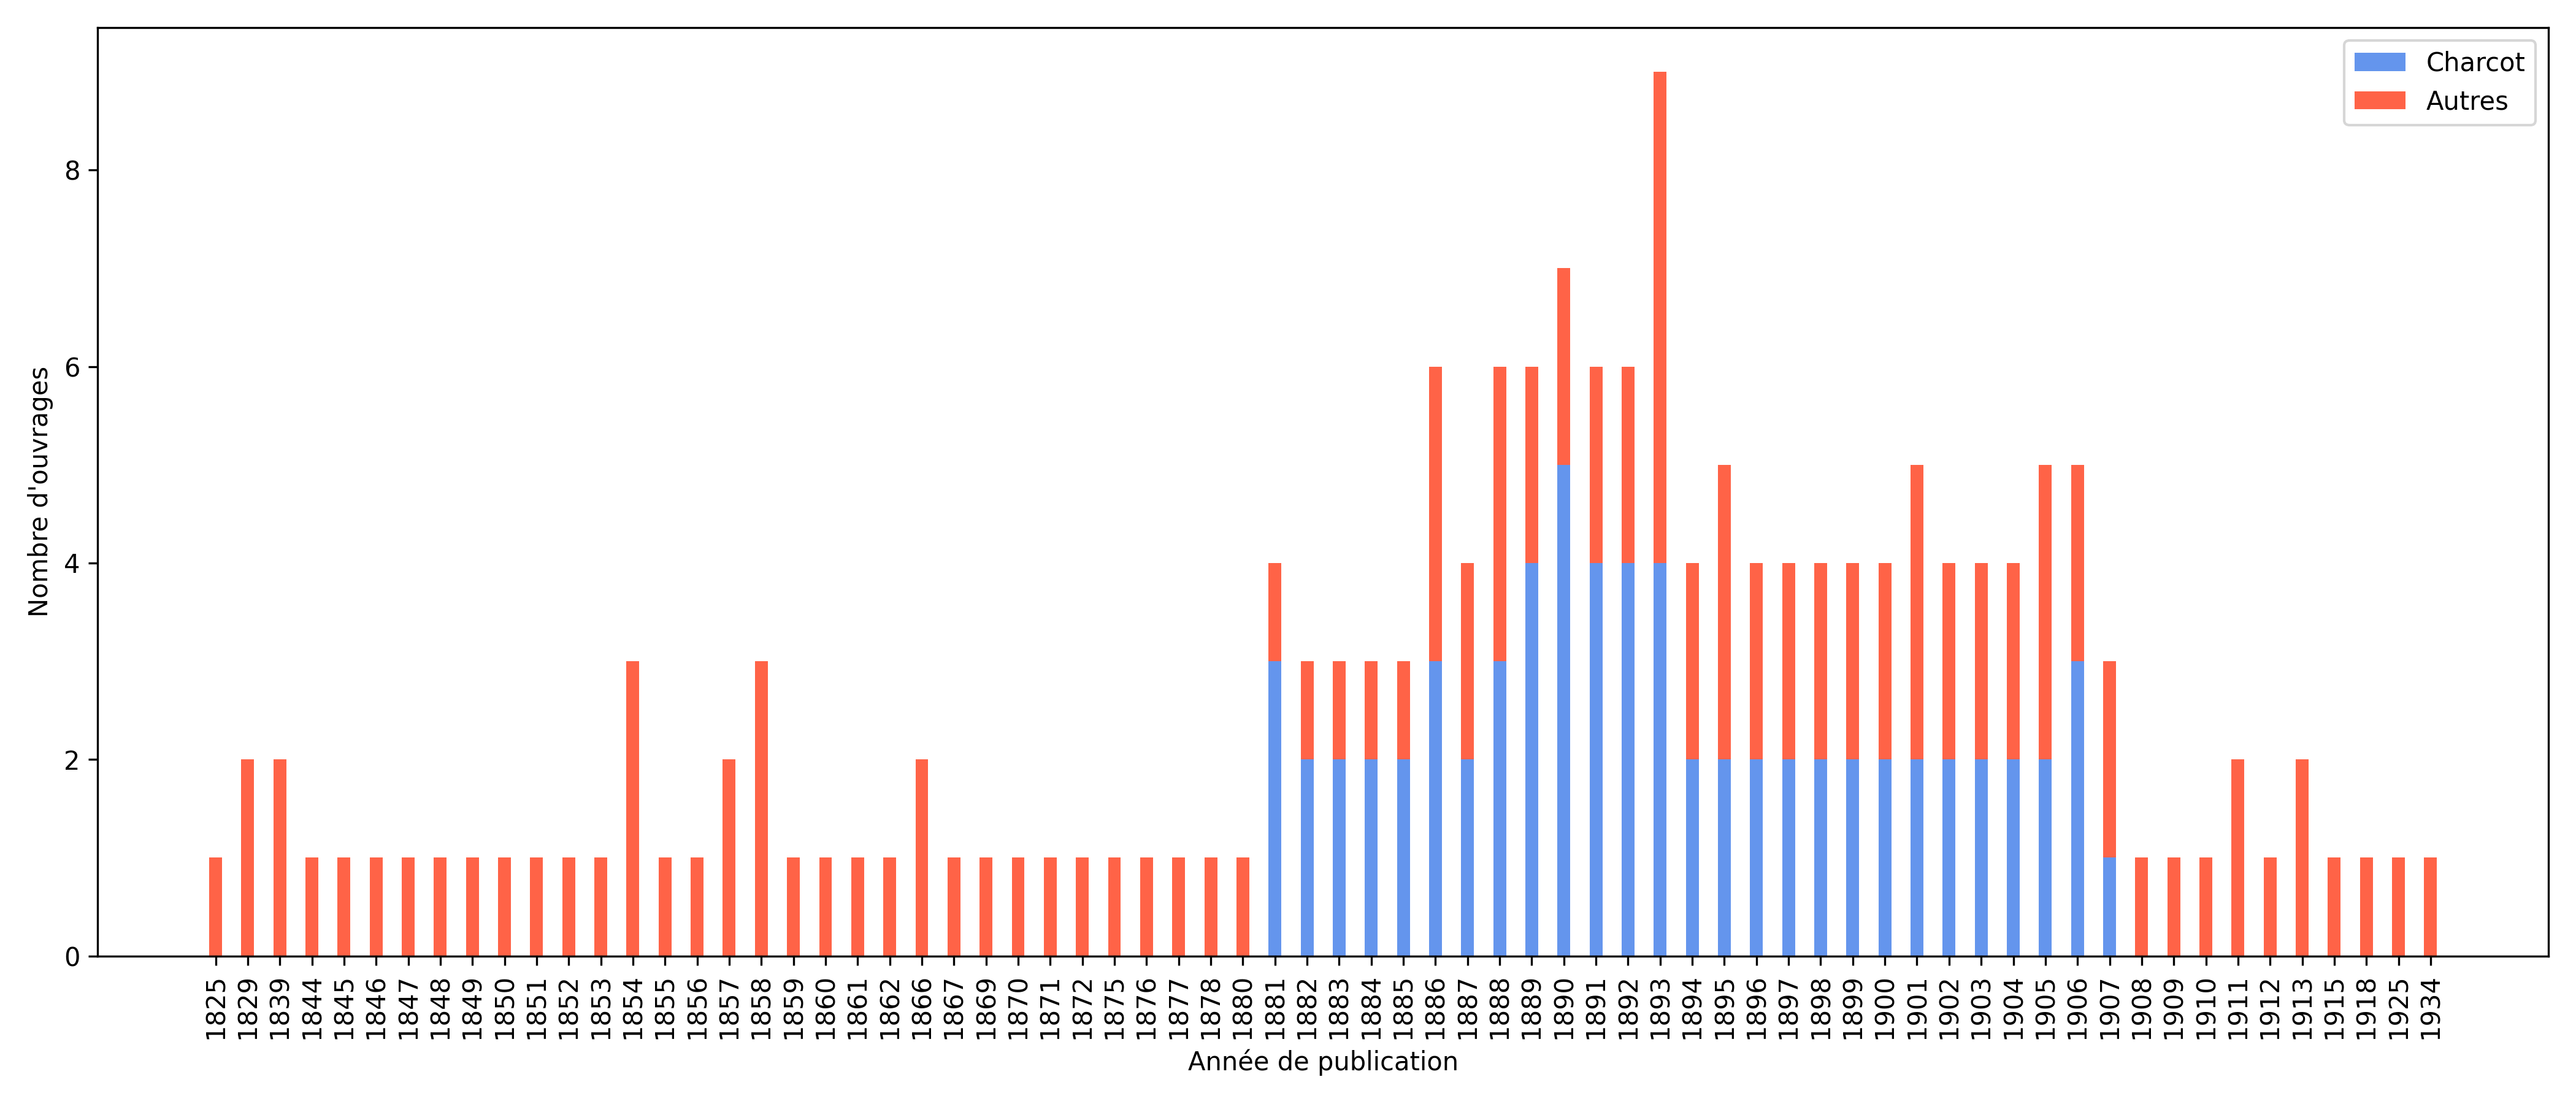
\includegraphics[width=1\textwidth]{img/distribution_ouvrages.png}
	\caption[Positionnement de l'entité \texttt{Jean-Martin Charcot} au sein de son domaine et comparaison avec les entités les plus similaires à lui \textit{via} une analyse de quadrant de l'outil Rankingdom.]{Répartition des ouvrages de Charcot et des Autres par année.}
	% Pour raison de visibilité, l'image originale a été agrandie, ce qui a entraîné le rapprochement des années sur l'axe de l'abscisse.
	\label{fig:repartition_corpus}
\end{figure}


\section{Historique de l'\textsc{ATR}}